\chapter{Results}
\label{ch:results}

	\section{Deforestation}
	\label{sec:results_deforestation}

		\subsection{Forest definition}
		\label{subsec:results_forest_definition}
		%TODO appendix graph distribution of the similarity indexes
		%TODO Bonferroni-Korrektur
			Our goal is to determine at which canopy cover density the agreement between \ac{GL30} and \ac{GFC} tree cover is greatest to receive the subsequent \ac{PDD} for stable \ac{LC} transitions introduced by anthropogenic causes. This process should ensure that we keep the largest number of tree cover loss samples from the \ac{GFC} dataset while harmonizing the tree cover definition between both layers. We applied the \ac{JI} to determine the similarity between each tile pair from our \ac{AISM}. The \ac{JI} computation is grouped by the continental regions Americas (82 tiles), Asia (86 tiles), and Africa (101 tiles). We determined the similarity for the following canopy density intervals: $(0, 100]$, $(10, 100]$, $(20, 100]$, and $(30, 100]$. Later we excluded all tiles with a initial \ac{JI} (canopy density intervall $(0,100]$) from our analysis because these tile pair does not contain any tree cover. We excluded 6, 9, and 15 tiles for Americas, Asia and Africa, respectively. To determine the canopy density interval where the agreement is at maximum we applied the non-parametric tests Wilcoxon signed-rank test and Wilcoxon rank-sum test. Both of the tests are performed as a one- and two-sided to deduce, if there is a difference in agreement (equality) and which direction (less or greater) has this difference. We applied continental and global testing to deduce regional differences and to determine the optimum for our subsequent \ac{PDD} predictions. Further, we compared the tree cover agreement of the three continental regions. Our initial hypothesis was that the tree cover agreement is at its maximum within the canopy density interval of $(30,100]$ for the entire study extent. We assumed that for the Americas and Asia the best results could be achieved with the same canopy density threshold. For Africa we assumed that the highest agreement could be achieved within the interval of $(10,100]$ because this region comprises a higher frequency of sparse woodland cover. The following paragraphs present our results for the three regions in the following order: Americas, Asia and Africa. The last paragraph discusses the results for the entire study extent and determines which canopy density we used for the following \ac{PDD} prediction.

			For Americas, Asia and Africa as well the entire study extent figure \ref{fig:jaccard} shows the distribution of the computed \acp{JI} for all tile pairs within the canopy density intervals. The x-axis are the different canopy density intervals where the label $JI_0$ accounts for $(0,100]$, $JI_1$ $(10,100]$, $JI_2$ $(20,100]$, and $JI_3$ $(30,100]$, respectively. The y-axis is the corresponding \ac{JI} between 0 and 1 where 0 highlights a complete disagreement and 1 a full agreement. The sample mean is labelled by a red cross and the boxes comprises the $Q_1$ (25 \%), $Q_2$ (50 \%), and $Q_3$ (75 \%) sample interval, respectively. For the Americas the sample mean does not change significantly within the four canopy density experiments. It is approximately 0.62 while sample median decreases from 0.68 to 0.66 from the interval class to the last. The upper 25 \% of the first experiment interval have a tree cover similarity ranging between approximately 0.8 and 1. This holds true over the other three experiments while only the maximum similarity slightly increases from 0.9787 to 0.9798. The figure \ref{fig:jaccard_americas_appendix} in the appendix suggests, that exclusions of canopy densities smaller than 11 increases slightly the tree cover agreement of the upper 25 \% but the exclusion of higher canopy density provides no benefit. This can be explained by the fact that the upper percentile already contain samples with a high tree cover agreement and it is to assume that only a small number of pixels have canopy density smaller than 30. Therefore, the interval change has only a small impact on this samples. For the first two canopy density intervals the range of the lower 25 \% percentile is between approximately 0.0003 and 0.45. Whereas the range increases from 0.0 to 0.5 for the last two interval classes. The figure \ref{fig:jaccard_americas_appendix} reveals a strong regional dependency of tree cover agreement within different canopy density classes of the lower percentiles. Whereas samples from the northern hemisphere show a decline in agreement the samples of the southern hemisphere show a increase of agreement. The strong up-shift of the southern samples within the last two intervals increases the range of lower percentile. This suggests in general that samples with low tree cover agreement benefit by the exclusion of lower canopy densities. The mobility of the samples within the $Q_1$ and $Q_3$ percentile show no general trend. For the first two experiments it ranges between 0.5 and 0.8 and for the last two it shows a small decline in $IQR$. This suggests that tiles within this group could benefit from a local optimisation of canopy density exclusion. We applied a Wilcoxon signed-rank test to deduce which canopy density class yields the highest tree cover agreement overall samples in the Americas. Table \ref{tab:wilcoxontwosided_regions} shows the results for the two-sided test and table \ref{tab:wilcoxontwosided_regions} for the one-sided test. The two-sided test reveals that only the similarity distribution between $JI_0$ and $JI_1$ is significantly different ($p<0.01$), while the comparison of the other distributions suggest that they are equal. The directional test of $JI_0$ and $JI_1$ suggests that the regional tree cover agreement is significantly greater ($p<0.005$) if canopy densities smaller than 10 are excluded. Additionally the table shows that $JI_2$ is significantly greater (p<0.05) than $JI_0$ but the comparison between $JI_1$ and $JI_2$ shows no significant difference. Therefore both tests confirm a strong regional or single tile agreement component. The directional test does not confirm that the distribution if $JI_1$ is significantly greater than $JI_2$ and $JI_3$. As the results of our experiments suggests is the tree cover agreement between \ac{GL30} and \ac{GFC} at canopy densities greater than 10 highest within the entire topical Americas. In case of local studies or for smaller extents the canopy density should be selected by a single tile approach to optimise the tree cover agreement by maximising the number of data points of the \ac{GFC} dataset.
			\begin{figure}[ht]
				\centering
				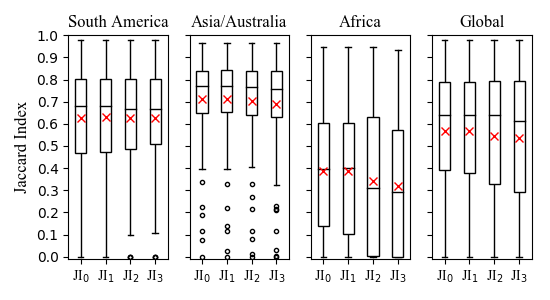
\includegraphics[scale=.91]{img/jaccard}
				\caption[Tree cover similarity distribution of the continental regions]{\textbf{Tree cover similarity distribution over the continental regions:} This boxplot shows the distribution of computed Jaccard Index for each raster image tile pair of GlobeLand30 and Global Forest Change tree cover from 2000. The labels $JI_0$, $JI_1$, $JI_2$, and $JI_3$ on the x-axis account for the canopy density classes (0,100], (10,100], (20,100], and (30,100], respectively. The y-axis is the computed Jaccard Index for the corresponding raster image pair, where 0 is a total disagreement and 1 a total agreement. Red crosses within the $Q_{25}$, $Q_{50}$, and $Q_{75}$ boxes highlight the sample mean. Whiskers are 1.5 times the $IQR$.}
				\label{fig:jaccard}
			\end{figure}
			\begin{table}[ht]
				\centering
				\caption[Regional two-sided Wilcoxon signed-rank test]{\textbf{Regional two-sided Wilcoxon signed-rank test:} This table shows, regional differences in the tree cover agreement by considering different canopy densities between GlobeLand30 and Global Forest Change at 2000. The classes $JI_0$, $JI_1$, $JI_2$, and $JI_3$ as row and column headings account for the canopy density classes (0,100], (10,100], (20,100], and (30,100], respectively. The test hypothesis is H$_0$: $X_1=X_2$ where $X_1$ is the column $JI_n$ class and $X_2$ the row $JI_n$ class. The significance is indicated by $p^{*}<0.05$, $p^{**}<0.02$, and $p^{***}<0.01$.}
				\label{tab:wilcoxontwosided_regions}
				\begin{tabular}{llllllllll}
					\hline
					& \multicolumn{3}{|c}{Americas} & \multicolumn{3}{|c|}{Asia} & \multicolumn{3}{c|}{Africa} \\
					Cls & JI$_0$ & JI$_1$ & JI$_2$ & JI$_0$ & JI$_1$ & JI$_2$ & JI$_0$ & JI$_1$ & JI$_2$ \\\hline
					JI$_0$ & - & - & - & - & - & - & - & - & - \\
					JI$_1$ & .00$^{***}$ & - & - & .72 & - & - & .22 & - & - \\
					JI$_2$ & .06 & .36 & - & .00$^{***}$ & .00$^{***}$ & - & .03$^{*}$ & .03$^{*}$  & - \\
					JI$_3$ & .16 & .50 & .60 & .00$^{***}$ & .00$^{***}$ & .00$^{***}$ & .00$^{***}$ & .00$^{***}$ & .00$^{***}$ \\\hline
				\end{tabular}
			\end{table}
			\begin{table}[ht]
				\centering
				\caption[Regional one-sided Wilcoxon signed-rank test]{\textbf{Regional one-sided Wilcoxon signed-rank test:} This table shows, the direction of regional differences in the tree cover agreement by considering different canopy densities between GlobeLand30 and Global Forest Change at 2000. The classes $JI_0$, $JI_1$, $JI_2$, and $JI_3$ as row and column headings account for the canopy density classes (0,100], (10,100], (20,100], and (30,100], respectively. The test hypothesis is H$_0$: $X_1\leq X_2$ and H$_0$: $X_2\geq X_1$ where $X_1$ is the column $JI_n$ class and $X_2$ the row $JI_n$ class. The significance is indicated by $p^{*}<0.05$, $p^{**}<0.025$, $p^{***}<0.01$, and $p^{\dagger}<0.005$.}
				\label{tab:wilcoxononesided_regions}
				\begin{tabular}{lllllllllllll}
					\hline
					& \multicolumn{4}{|c}{Americas} & \multicolumn{4}{|c|}{Asia} & \multicolumn{4}{c|}{Africa} \\
					Cls & JI$_0$ & JI$_1$ & JI$_2$ & JI$_3$ & JI$_0$ & JI$_1$ & JI$_2$ & JI$_3$ & JI$_0$ & JI$_1$ & JI$_2$ & JI$_3$ \\\hline
					JI$_0$ & - & .00$^{\dagger}$ & .03$^{*}$ & .08 & - & .64 & 1. & 1. & - & .11 & .98 & 1. \\
					JI$_1$ & 1. & - & .18 & .25 & .36 & - & 1. & 1. & .89 & - & .99 & 1. \\
					JI$_2$ & .97 & .82 & - & .30 & .00$^{\dagger}$ & .00$^{\dagger}$ & - & 1. & .02$^{**}$ & .01$^{**}$ & - & 1. \\
					JI$_3$ & .92 & .75 & .70 & - & .00$^{\dagger}$ & .00$^{\dagger}$ & .00$^{\dagger}$ & - & .00$^{\dagger}$ & .00$^{\dagger}$ & .00$^{\dagger}$ & - \\\hline
				\end{tabular}
			\end{table}

			For Asia, the sample mean scatters around 0.7 as the red crosses in figure \ref{fig:jaccard} suggest. The sample mean decreases slightly at higher canopy density intervals. Further, the median is approximately 0.8 by showing a slight decrease at higher canopy density intervals too. The range of the upper percentiles for all experiments groups is between approximately 0.85 and 0.96 while the maximum agreement decreases slightly from 0.9654 to 0.9634. Figure \ref{fig:jaccard_asia_appendix} in the appendix, reveals that in general the tree cover agreement increases if canopy densities below 10 \% are excluded but the exclusion of densities above 20 \% reverts this. For Asia the lower percentile ranges between approximately 0 and 0.65 while most of the samples show a decline in tree cover agreement if canopy densities above 20 are excluded. Within the $Q_1,3$ percentile a per tile relationship is detectable. The range of this percentile is between 0.65 and 0.85 for the first two classes $JI_0$ and $JI_1$ while the range increases for the last two experiments. As mentioned no clear trend is observable some of the samples benefit if the considered canopy density interval is increased till 30 \% and some show a decrease in agreement if the canopy density is lift over 10 \%. The two-sided Wilcoxon test in table \ref{tab:wilcoxontwosided_regions} reveals that the similarity distribution is significantly different (p<0.01) between each experiment group except the pair of $JI_1$ and $JI_0$. The directional test in table \ref{tab:wilcoxononesided_regions} reveals that the tree cover agreement distributions of $JI_2$ and $JI_3$ are significantly smaller than $JI_0$ and $JI_1$ (p<0.005). Further this results show that the distributions of $JI_0$ and $JI_1$ have no directional differences. This could be explained by a regional or tile-wise agreement component. While some of the tiles show strong increase in similarity if canopy density is set to 10 \%, others show a decrease. A more detailed analysis could be performed by applying a smaller canopy density step-size. For studies targeting the region Asia the results of the directional tests suggest to use all data from \ac{GFC} within the canopy density interval of $(0,100]$. While the figure \ref{fig:jaccard_asia_appendix} suggests to include all data form the interval $(10,100]$.

			\note{Africa (review):} As figure \ref{fig:jaccard} for Africa suggests is the similarity distribution mobility of the samples in Africa at highest. The first two similarity distributions have an comparable mean and median at 0.38 and 0.4. The last two classes show a strong decline in mean and median to approximately 0.33 and 0.3. The mobility of the upper 25 percent of the first two canopy density classes is already quite strong as figure appendix suggests. While the iqr range for $JI_0$ is between 0.15 and 0.6 the range increases for the second $JI_1$ by connecting to more agreement downwards trend. The tile pairs in africa are characterized by 17 (approx. 20 percent) where the tree cover agreement is smaller than 0.1. 11 of these tiles have already a agreement of 0.0 when the first canopy density is excluded. These trend continues as more canopy density is excluded as more samples have a agreement of 0.0. This explains the high iqr range for the canopy densities exclusion greater than 10 percent. At $JI_3$ already two fifth (42 percent) of the samples have an tree cover agreement lower than 0.1. The two sided wilcoxon test shows that the distribution of $JI_2$ and $JI_3$ significantly differs (p<0.05 and p<0.01). As the table suggest is the distribution of $JI_0$ and $JI_1$ nearly the same. The one sided test reveals that reducing the canopy density below 10 percent decreases the tree cover agreement between sample distributions. For $JI_0$ and the $JI_1$ the test reveals that no clear trend is detectable. Appendix figure shows that some samples benefit from the exclusion of canopy density and as mentioned some samples show a strong decrease in tree cover similarity. As the data shows is the regional dependency of tree cover agreement at largest. To maximize the similarity on continental level for africa it should the entire data range of Global Forest Change should be slected. It could also be also a solution to select canopy densities in the interval 10 to 100 but here the trade is to have tiles where no tree cover agreement is detectable.

			\note{Comparison between regions (review):} Table appendix shows that Asia has the highest tree cover similarity distribution over all regions within all tested canopy classes followed by the Americas for GlobeLand30 and Hansen 2000. Africa has the poorest tree cover agreement within our tested regions. As discussed in the previous paragraphs the reason could be that Americas and Asia have mainly core tropical forest zones where the forest cover is dense and the canopy density is above 30 percent. This can be highlighted by section tropical deforestation and the shown tree cover maps. Africa in comparison to Asia and Americas has large zones where the tree cover is high but the canopy density is low also described by the term sparse woodland. As it looks these sparse woodlands compete the forest detection methods of both datasets. This fact could lead within the hansen dataset to ghost deforestation because it is hard to detect sparse woodland it could be the annual deforestation does not detect it as forest and it is recognized as deforestation. Therefore in africa the rationality of tree cover agreement must be considered during preparation and validation of studies. Also it is to suggest to optimize tree cover agreement on regional scale and not over the entire continent. Overall regions the upper 25 percent of the samples benefit or shown only small changes if the canopy density is increased.

			On the far right of figure \ref{fig:jaccard} the tree cover agreement of the entire study extent is presented. The sample mean and median differ between the first two experiment groups and the last two groups. For the first two groups the mean and median account for 0.56 and 0.63, respectively. The last two experiment groups show a decline to 0.53 and 0.53 for mean and median. For the upper percentile the same statement as for the regions holds true. In general, the samples with high tree cover agreement benefit from the exclusion of lower canopy densities. The lower percentile shows strong regional or tile-wise tree agreement dependencies. If we consider the entire sample range the mid percentile steadily increases its range from 0.4 to 0.8 till 0.3 to 0.8. As mentioned in the regional analysis, this percentile is characterized by inhomogeneous changes of tree cover agreement by the step-wise change of the canopy density. In general the trend points downwards as the decrease in median and the range increase show. The results of the two-sided Wilcoxon test in table \ref{tab:wilcoxontwosided_all} show a significant difference in distribution (p<0.02 and p<0.01) between each experiment group except $JI_0$ and $JI_2$ where the similarity distribution could be the same. Table \ref{tab:wilcoxononesided_all} highlights the directional component of these distribution differences. At a global scale the tree cover agreement is at its maximum if we set the canopy density interval to $(10,100]$. The second experiment group $JI_1$ is significantly greater than $JI_0$ (p<0.005) and the last two groups $JI_2$ and $JI_3$ are significantly smaller (p>0.005) than $JI_1$. Further, the tree cover agreement of $JI_0$ is significantly greater than (p<0.005 and p<0.05) $JI_2$ and $JI_3$. Therefore it is proved that canopy densities above 20 \% reduce the tree cover agreement between \ac{GL30} and \ac{GFC} on a global level. On a global scale as the analysis on tree cover agreement suggests the highest agreement can be achieved within the $JI_1$ interval. Therefore we decided to proceed for our study of \ac{PDD} and the derived products with this definition of tree cover. \note{To clarify we filtered the \ac{GFC} with this canopy density definition and superimposed gl30 and....}
			\begin{table}[ht]
				\centering
				\caption[Global two-sided Wilcoxon signed-rank test]{\textbf{Regional two-sided Wilcoxon signed-rank test:} This table shows, global differences in the tree cover agreement by considering different canopy densities between GlobeLand30 and Global Forest Change at 2000. The classes $JI_0$, $JI_1$, $JI_2$, and $JI_3$ as row and column headings account for the canopy density classes (0,100], (10,100], (20,100], and (30,100], respectively. The test hypothesis is H$_0$: $X_1=X_2$ where $X_1$ is the column $JI_n$ class and $X_2$ the row $JI_n$ class. The significance is indicated by $p^{*}<0.05$, $p^{**}<0.02$, and $p^{***}<0.01$.}
				\label{tab:wilcoxontwosided_all}
				\begin{tabular}{llll}
					\hline
					Cls & JI$_0$ & JI$_1$ & JI$_2$ \\\hline
					JI$_0$ & - & - & - \\
					JI$_1$ & .00$^{***}$ & - & - \\
					JI$_2$ & .08 & .02$^{**}$ & - \\
					JI$_3$ & .00$^{***}$ & .00$^{***}$ & .00$^{***}$ \\\hline
				\end{tabular}
			\end{table}
			\begin{table}[ht]
				\centering
				\caption[Global one-sided Wilcoxon signed-rank test]{\textbf{Global one-sided Wilcoxon signed-rank test:} This table shows, the direction of global differences in the tree cover agreement by considering different canopy densities between GlobeLand30 and Global Forest Change at 2000. The classes $JI_0$, $JI_1$, $JI_2$, and $JI_3$ as row and column headings account for the canopy density classes (0,100], (10,100], (20,100], and (30,100], respectively. The test hypothesis is H$_0$: $X_1\leq X_2$ and H$_0$: $X_2\geq X_1$ where $X_1$ is the column $JI_n$ class and $X_2$ the row $JI_n$ class. The significance is indicated by $p^{*}<0.05$, $p^{**}<0.025$, $p^{***}<0.01$, and $p^{\dagger}<0.005$.}
				\label{tab:wilcoxononesided_all}
				\begin{tabular}{lllll}
					\hline
					Cls & JI$_0$ & JI$_1$ & JI$_2$ & JI$_3$ \\\hline
					JI$_0$ & - & .00$^{****}$ & .96 & 1. \\
					JI$_1$ & 1. & - & .99 & 1. \\
					JI$_2$ & .04$^{*}$ & .01$^{***}$ & - & 1. \\
					JI$_3$ & .00$^{****}$ & .00$^{****}$ & .00$^{****}$ & - \\\hline
				\end{tabular}
			\end{table}

		\subsection{Tree cover and deforestation}
		\label{subsec:results_tree_cover_and_deforestation}
		%TODO images of loss and canopy
			\note{Goal (review):} This section is intended to show the distribution of tree cover within our study extent as well to present at which places the loss of tree cover has is main impacts in the tropical zone. The tree cover map is derived from the \ac{GFC} tree cover 2000 dataset while we selected only forest within our canopy density interval $(10,100]$. To present the tree cover we use our hexagonal binning approach. We compute the total area covered by trees within a hexagon and divide by the total area a hexagon occupies to get the scaling. Additionally we determine the mean canopy density per hexagon. To arrange the loss maps we use our proximate deforestation driver predictions. We compute for each hexagon the area which is lost by deforestation drivers classified as antrophogenic. We divide this by the total area a hexagons covers to determine the scaling. This map should be interpreted as additionally information to our predictions and as a example how large data can be visualized by an easy reproduceable approach.

		\subsection{Proximate deforestation driver}
		\label{subsec:results_proxy_deforestation_driver}
			\note{Goal (review):}

		\subsection{Accuracy assessment}
		\label{subsec:results_accuracy_assessment}
		%TODO distribution is it in line with global estimates
		
			\note{Goal (review):} Goal is the assessment of the accuracy of our proximate deforestation driver predictions. We created a set of ground truth data by sampling our proximate deforestation driver layers. In each region we select per random 10 tiles and draw 200 samples per tile. The 200 samples comprises pixels over the full value range of our proximate deforestation driver classes. We imported the prepared sample to our JavaScript application and subsequently classified each sample with a label. To determine the accuracy we used a confusion matrix and the derived metrics like producers accuracy, overall accuracy, kappa coefficient etc.

			\note{Results (review):} Table \ref{tab:results_confusion_matrix} shows the confusion matrix to determine the accuracy of our predictions where the term reference refers to the labeling of pixel by our visual interpretation and predictions refer to the labeling of our proximate driver predictions. The abbreviations PAc, UAc, OvAc, Com, Om, Tot, and Kappa refer to the terms Producers-Accuracy, Users-Accuracy, Overall-Accuracy, Error of Commission, Error of Omission, row or column total, and Kappa Coefficient. From the 6000 samples we draw from our study extent 14 \%, 20 \%, 22 \%, 32 \%, 8 \%, 2 \%, 0.5 \%, 2 \%, and 0.5 \% account for cultivated land (10), tree cover (20), regrowth (25), shrubland (40), wetland (50), water (60), artificial land (80), and bareland (90), respectively. Our method predicts a distribution of 15 \%, 18 \%, 27 \%, 31 \%, 7 \%, 1 \%, 0.8 \%, 1 \%, and 0.2 \% for the land cover classes 10, 20, 25, 30, 40, 50, 60, 80, and 90, respectively.
			Highest producers accuracy is achieved the regrowth class with 88 percent. The prediction of this class was achieved by including global forest change gain data within our target canopy density. During building our reference data set per visual interpretation we determined this class by following these rules. We checked the surroundings and the corresponding pixel for signs of road networks and infrastructure. Further we checked if the canopy shows signs of age class forest and line patterns which show the establishment of artificial introduced forest cover. During the visual interpretation we recognized that a large portion of the regrowth class is occupied by plantations especially in Americas and Asia. For Asia a major share was occupied by palm oil or other plantations. It must be mentioned that here the deforestation within our temporal frame is not coercively the clearing of natural cover/primary forest it shows it shows also rotational cycles of deforestation reforestation.
			The second highest accuracy with 85 (producers accuracy) was achieved in the prediction of cultivated land where only 15 percent could be identified as error of commission. 8.2 percent are classified as forest or regrowth which could reveal zones of shifting agriculture or temporal issues. To identify this class during our visual interpretation we applied nearly the same rules as the detection of regrowth checking for infrastructure but here no canopy should be identified. Further we checked for large scale square patterns which is shown by large scale commodity driven agriculture. Especially the small scale agriculture was hard detect because these class of agriculture often show no regular patterns of forest clearing and are often accompanied by selective logging. Further it should be mentioned common practice of small scale agriculture is inhomogeneous over the regions Americas, Asia and Africa. Another good indicator for cultivated land is the appearance of tillage patterns on high resolution imagery. Cultivated land comprises a large variety of different use cases. 
			Grassland shows an accuracy of 77 at an error of commission of 23 percent. The error could lead back to classification errors by GlobeLand30 or land cover change dynamics and the temporal time frame. For visual interpretation cultivated land and grassland share some common properties like square shaped clearings and infrastructure in the surroundings. But grassland is also defined by the occurrence of shrubs and single trees within its extent. To really determine the differences between both classes high resolution imagery is required. In Americas the grassland patches could often be identified as used for cattle ranching. During visual interpretation we recognized frequently the occurrence of water holes. Africa showed the occurrence of natural grasslands and Asia bla.

			\begin{table}[ht]
				\centering
				\caption[Confussion matrix]{\textbf{Confussion matrix for accuracy assessment:} We draw 6000 samples from 10 random selected tiles from the three regions Americas, Asia and Africa. Labels refer to our proximate deforestation driver classes which correspond to GlobeLand30 classification schema in table \ref{tab:gl30_classes}. Reference refers to the samples we classified by visual interpretation of external imagery and predictions refer to the label the sample has in our proximate driver product. The abbreviations PAc, UAc, OvAc, Com, Om, Tot, and Kappa refer to the terms Producers-Accuracy, Users-Accuracy, Overall-Accuracy, Error of Commission, Error of Omission, row or column total, and Kappa Coefficient.}
				\label{tab:results_confusion_matrix}
				\begin{tabular}{llrrrrrrrrrrrr}
					\hline
					& & \multicolumn{9}{c}{Reference} & & & \\\cline{3-11}
					& Cls & 10 & 20 & 25 & 30 & 40 & 50 & 60 & 80 & 90 & Tot & UAc & Om \\\hline
					\multirow{9}{*}{\STAB{\rotatebox[origin=c]{90}{Prediction}}}
					& 10 & 730 & 37 & 62 & 15 & 16 & 2 & 3 & 5 & 0 & 870 & .84 & .16 \\ 
					& 20 & 41 & 744 & 56 & 189 & 31 & 12 & 0 & 15 & 4 & 1092 & .68 & .32 \\ 
					& 25 & 29 & 202 & 1155 & 172 & 22 & 10 & 5 & 11 & 4 & 1610 & .72 & .28 \\ 
					& 30 & 36 & 187 & 32 & 1466 & 73 & 21 & 0 & 17 & 0 & 1832 & .80 & .20 \\ 
					& 40 & 14 & 21 & 4 & 41 & 352 & 1 & 1 & 2 & 1 & 437 & .81 & .19 \\ 
					& 50 & 0 & 5 & 3 & 10 & 4 & 50 & 0 & 1 & 0 & 73 & .68 & .32 \\ 
					& 60 & 2 & 1 & 0 & 3 & 0 & 2 & 18 & 2 & 0 & 28 & .64 & .36 \\ 
					& 80 & 3 & 3 & 0 & 1 & 1 & 1 & 0 & 40 & 0 & 49 & .82 & .18 \\ 
					& 90 & 0 & 0 & 0 & 1 & 0 & 0 & 0 & 3 & 5 & 9 & .56 & .44 \\\hline 
					& Tot & 855 & 1200 & 1312 & 1898 & 499 & 99 & 27 & 96 & 14 & 6000 & & \\
					& PAc & .85 & .62 & .88 & .77 & .71 & .51 & .67 & .42 & .36 & Kappa & \multicolumn{2}{r}{OvAc} \\
					& Com & .15 & .38 & .12 & .23 & .29 & .49 & .33 & .58 & .64 & .69 & \multicolumn{2}{r}{.76} \\ \hline
				\end{tabular}
			\end{table}

	\section{Emissions}
		\note{Goal (review):}

	\section{Ecosystem service values}
	%TODO compute global balance
	%TODO compute regional balance
	%TODO country table goes to appendix
	%TODO aggregate per
		Our goal is to estimate the monetary loss of \ac{ESV} by \ac{PDD} at a global, continental, and regional scale. Additionally, we approximated the monetary gain if tree cover is converted to a certain type of \ac{LC}. We refer to this gain as \ac{ESV} gain. Further, we computed the balance between \ac{ESV} loss and gain to estimate the net change of \ac{ESV} in the tropical zone. We applied three datasets which estimate the monetary value of ecosystems on a global scale namely the following data: \citet{Groot2012}, \citet{Costanza2014}, and \citet{Siikamaki2015}. To compute the monetary loss of \ac{ESV} we selected the following \ac{PDD} classes as anthropogenic deforestation: 10 (cultivated land), 25 (regrowth), 30 (grassland), 40 (shrubland), 80 (artificial land), and 90 (bareland). The \ac{ESV} gain depends on the particular \ac{ESV} dataset because the datasets don't define a monetary value for each \ac{PDD} class. For detailed informations refer to section \ref{subsec:esv_methods}. The \ac{ESV} net change or balance is the difference of \ac{ESV} loss and gain. The monetary unit for each value is the Geary–Khamis dollar at 2007 also known as international dollar (2007 Int.\$ ha$^{-1}$).

%%%%%%% TABLE AND FIGURES

%			\begin{table}[ht]
%				\centering
%				\caption[Deforestation driver]{Absolute in km$^2$}
%				\label{tab:driver_tab}
%				\begin{tabular}{lcllrrr}
%					Class & Code & Type & & Americas & Asia & Africa \\\hline
%					\multirow{4}{*}{Agriculture} & \multirow{2}{*}{10} & \multirow{2}{*}{Cropland} & rel. & 24.37 & 18.37 & 25.01 \\
%					& & & abs. & 95908 & 38719 & 44368 \\
%					& \multirow{2}{*}{30} & \multirow{2}{*}{Grassland} & rel. & 46.19 & 8.41 & 50.46 \\
%					& & & abs. & 181781 & 17726 & 89516 \\
%					\multirow{4}{*}{Forestry/Plantations} & \multirow{2}{*}{25} & \multirow{2}{*}{Regrowth} & rel. & 14.40 & 70.27 & 18.61 \\
%					& & & abs. & 56671 & 148111 & 33014 \\
%					& \multirow{2}{*}{40} & \multirow{2}{*}{Shrubland} & rel. & 12.69 & 1.11 & 3.77 \\
%					& & & abs. & 49941 & 2340 & 6688 \\
%					\multirow{4}{*}{Urban/Mining} & \multirow{2}{*}{80} & \multirow{2}{*}{Artificial} & rel. & 0.41 & 0.46 & 0.71 \\
%					& & & abs. & 1614 & 970 & 1260 \\
%					& \multirow{2}{*}{90} & \multirow{2}{*}{Bareland} & rel. & 0.10 & 0.03 & 0.09 \\
%					& & & abs. & 394 & 63 & 160 \\
%					\multirow{4}{*}{Natural} & \multirow{2}{*}{50} & \multirow{2}{*}{Wetland} & rel. & 1.50 & 0.97 & 1.23 \\
%					& & & abs. & 5903 & 2045 & 2182 \\
%					& \multirow{2}{*}{60} & \multirow{2}{*}{Water} & rel. & 0.32 & 0.38 & 0.13 \\
%					& & & abs. & 1259 & 801 & 231 \\\hline
%					\multicolumn{3}{c}{\multirow{2}{*}{Forest loss}} & rel. & 3.87 & 4.68 & 1.69 \\
%					& & & abs. & 393550 & 210774 & 177400 \\
%					\multicolumn{3}{c}{Forest cover} & abs. & 10223187 & 4457940 & 10496591 \\\hline
%				\end{tabular}
%			\end{table}

% LATIN AMERICA
%			\begin{figure}[ht]
%				\centering
%				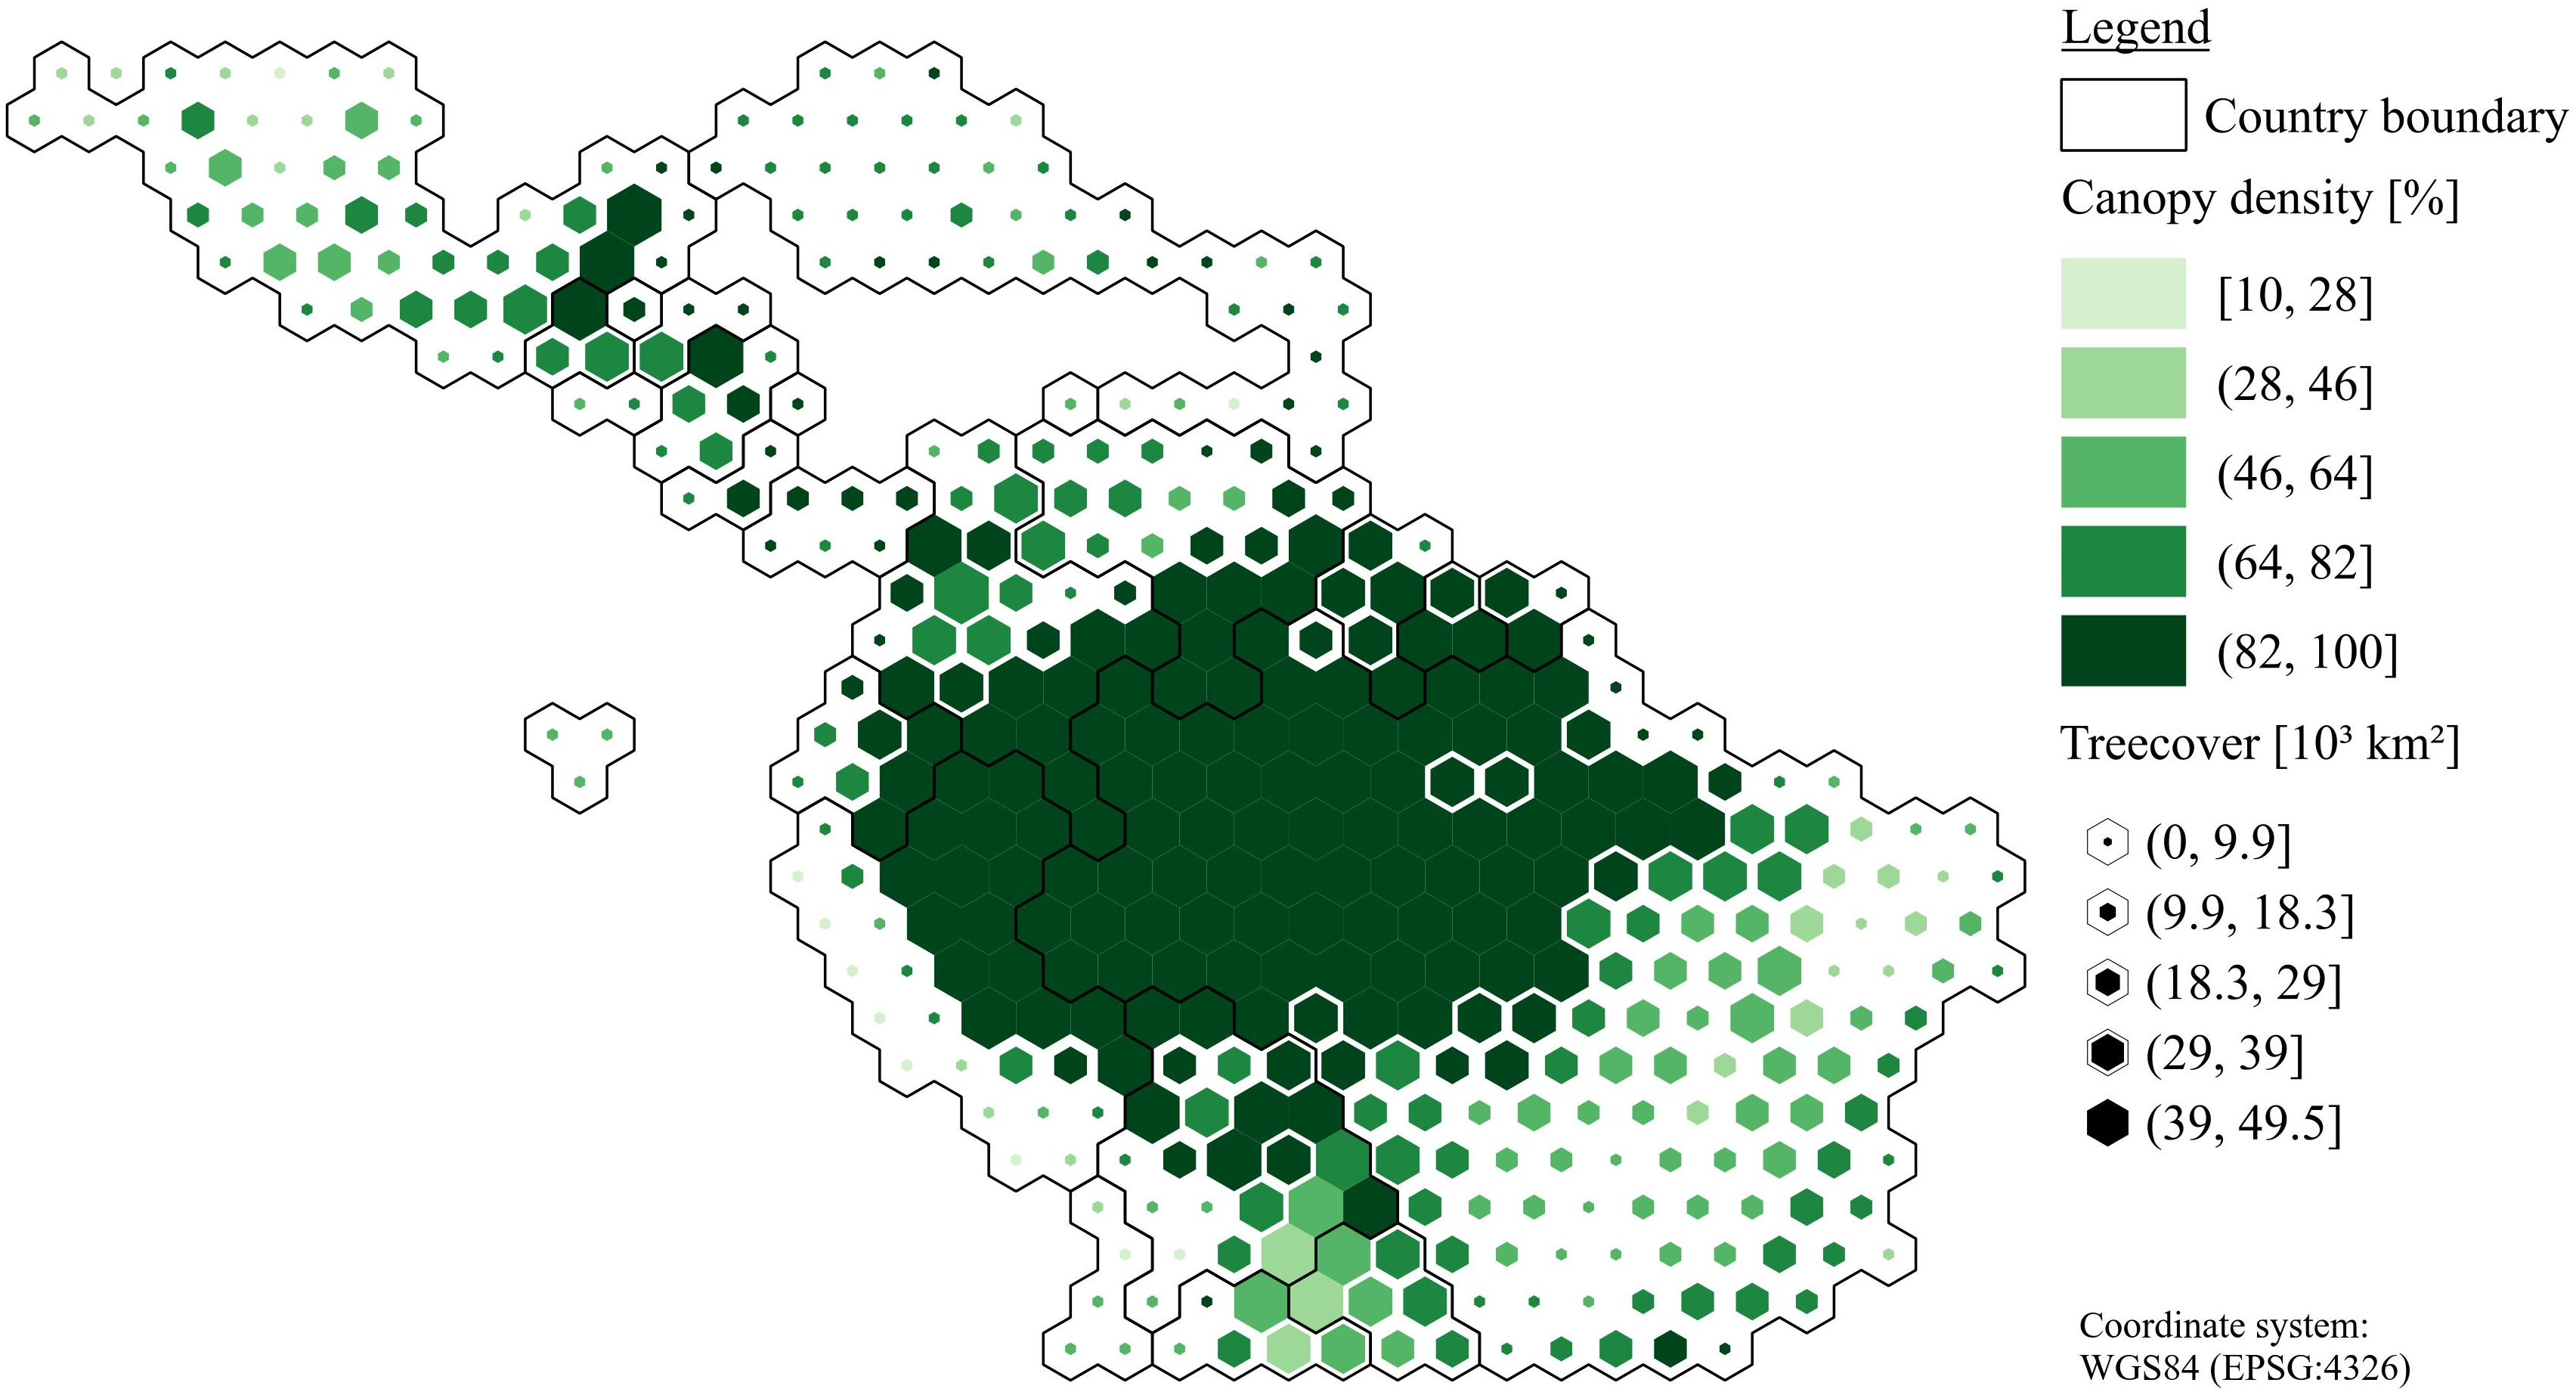
\includegraphics[scale=1]{img/americas_treecover_frameless}
%				\caption[Ecosystem service values]{}
%				\label{fig:americascover}
%			\end{figure}
%			\begin{figure}[ht]
%				\centering
%				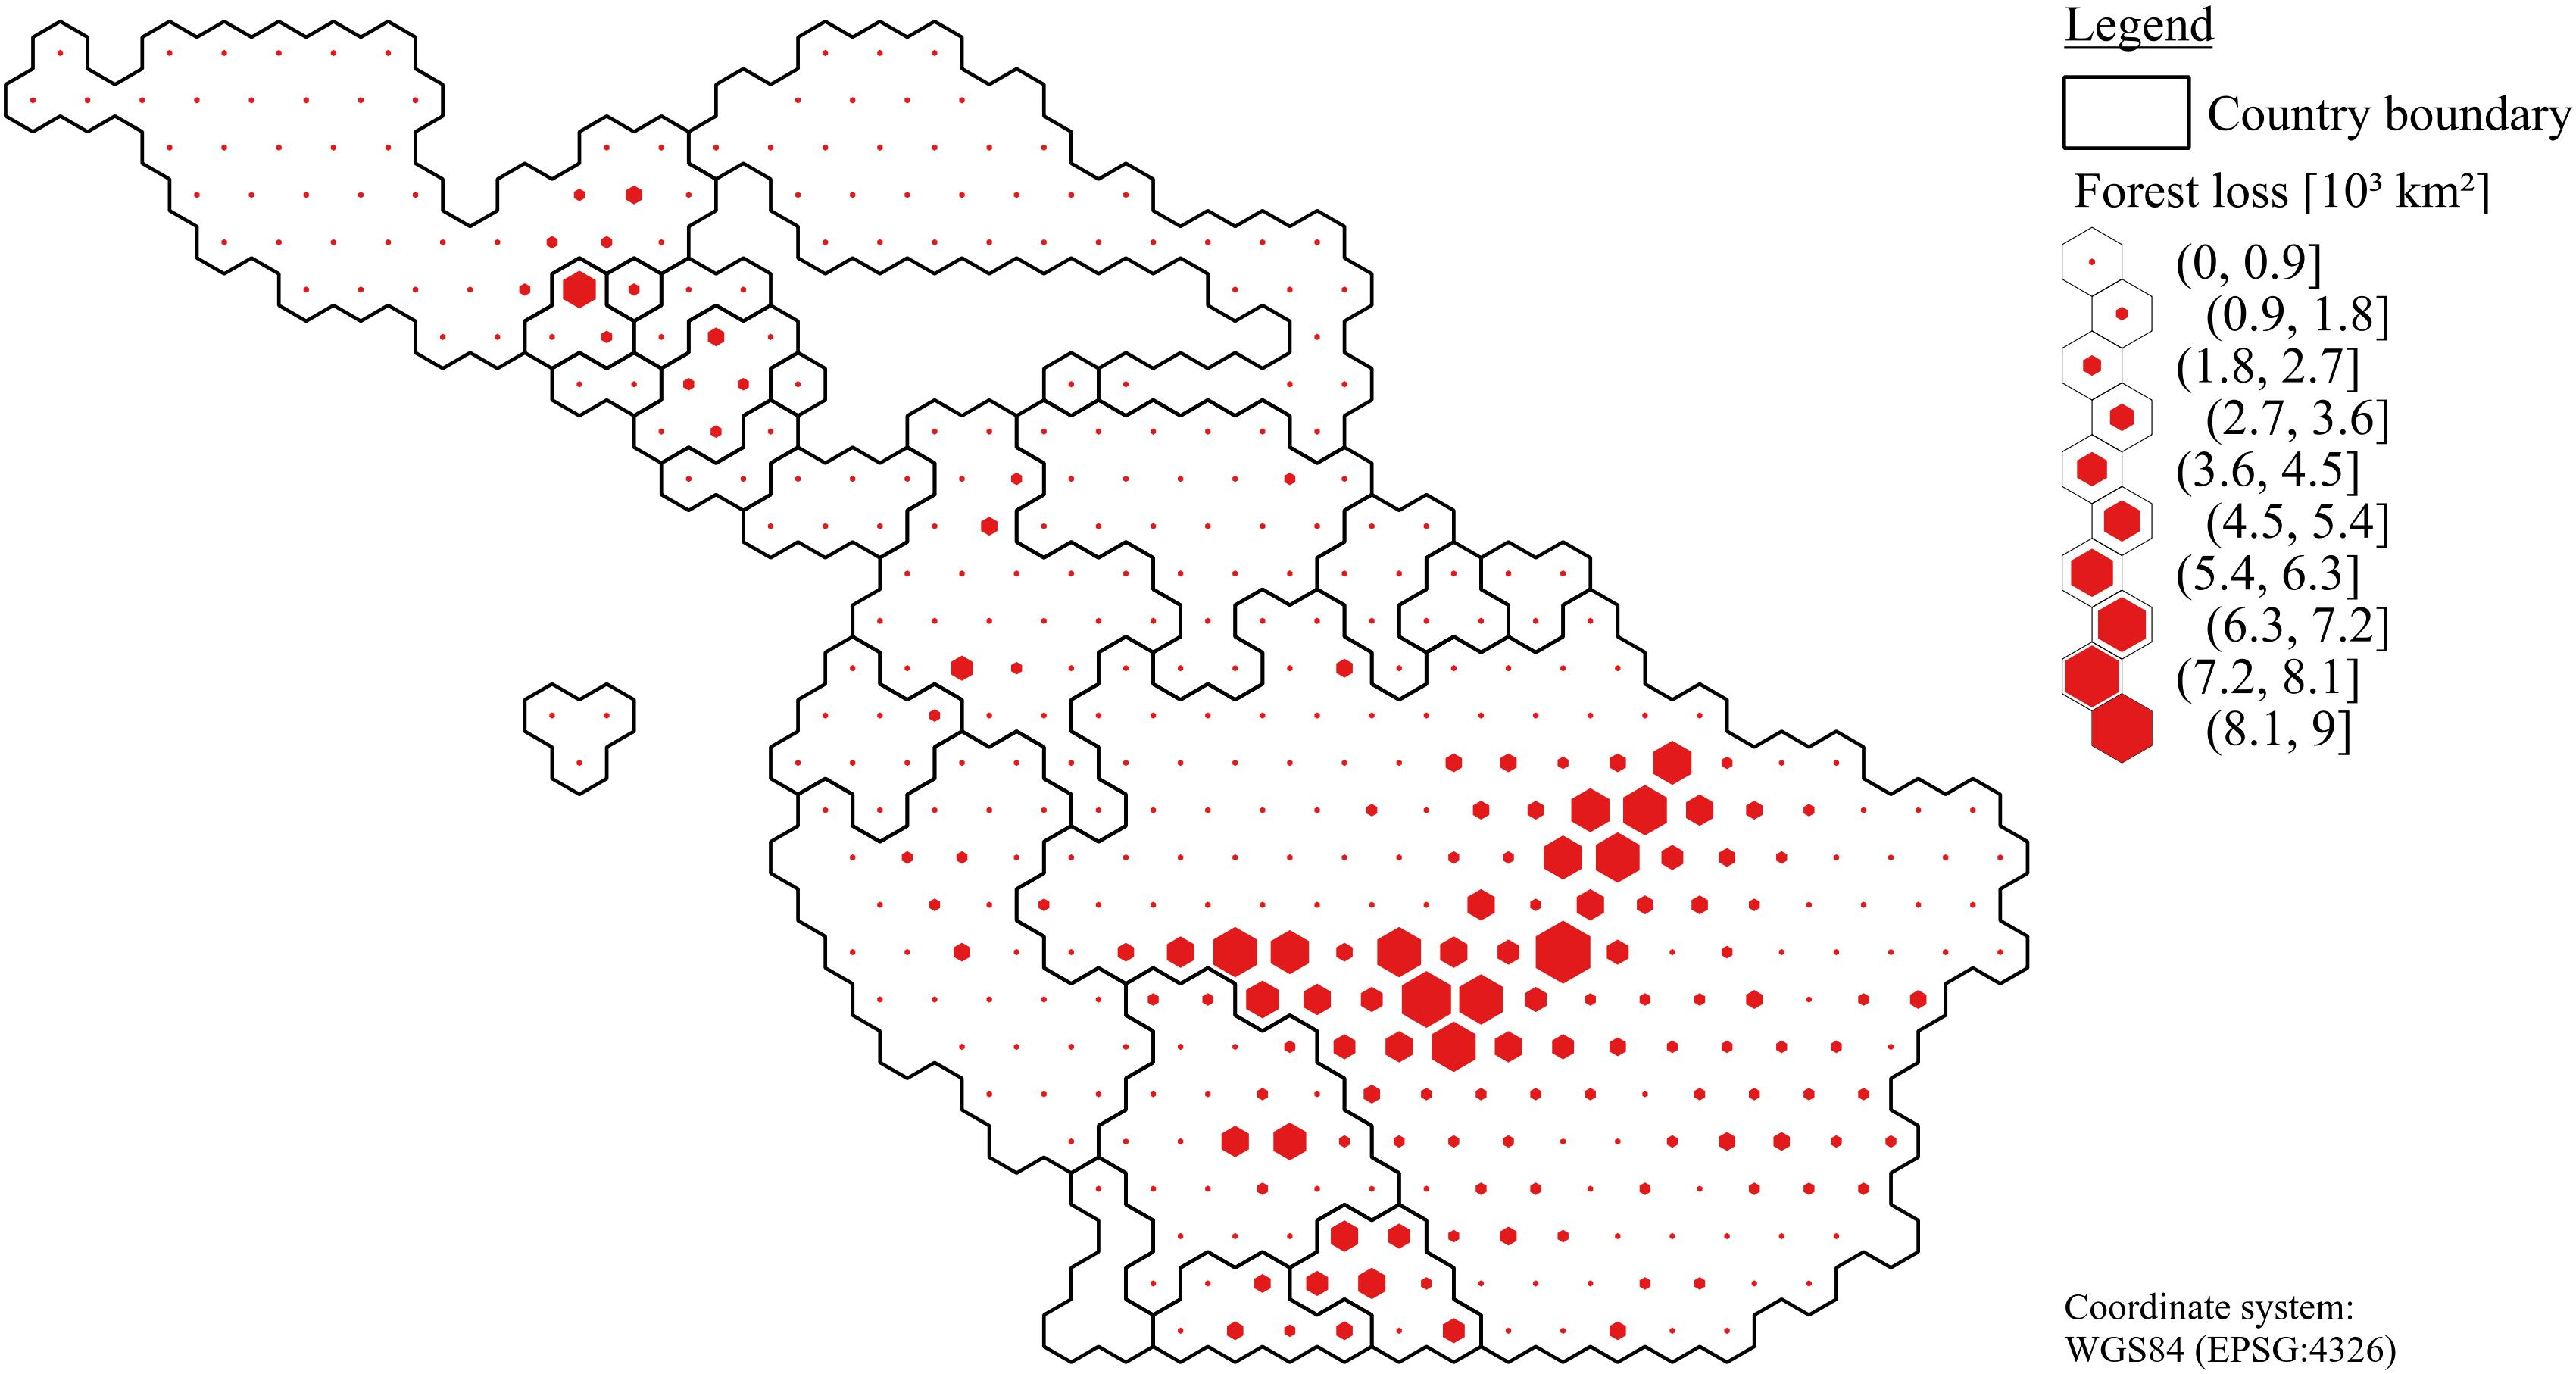
\includegraphics[scale=1]{img/americas_loss_frameless}
%				\caption[Ecosystem service values]{}
%				\label{fig:americasloss}
%			\end{figure}
%			\begin{figure}[ht]
%				\centering
%				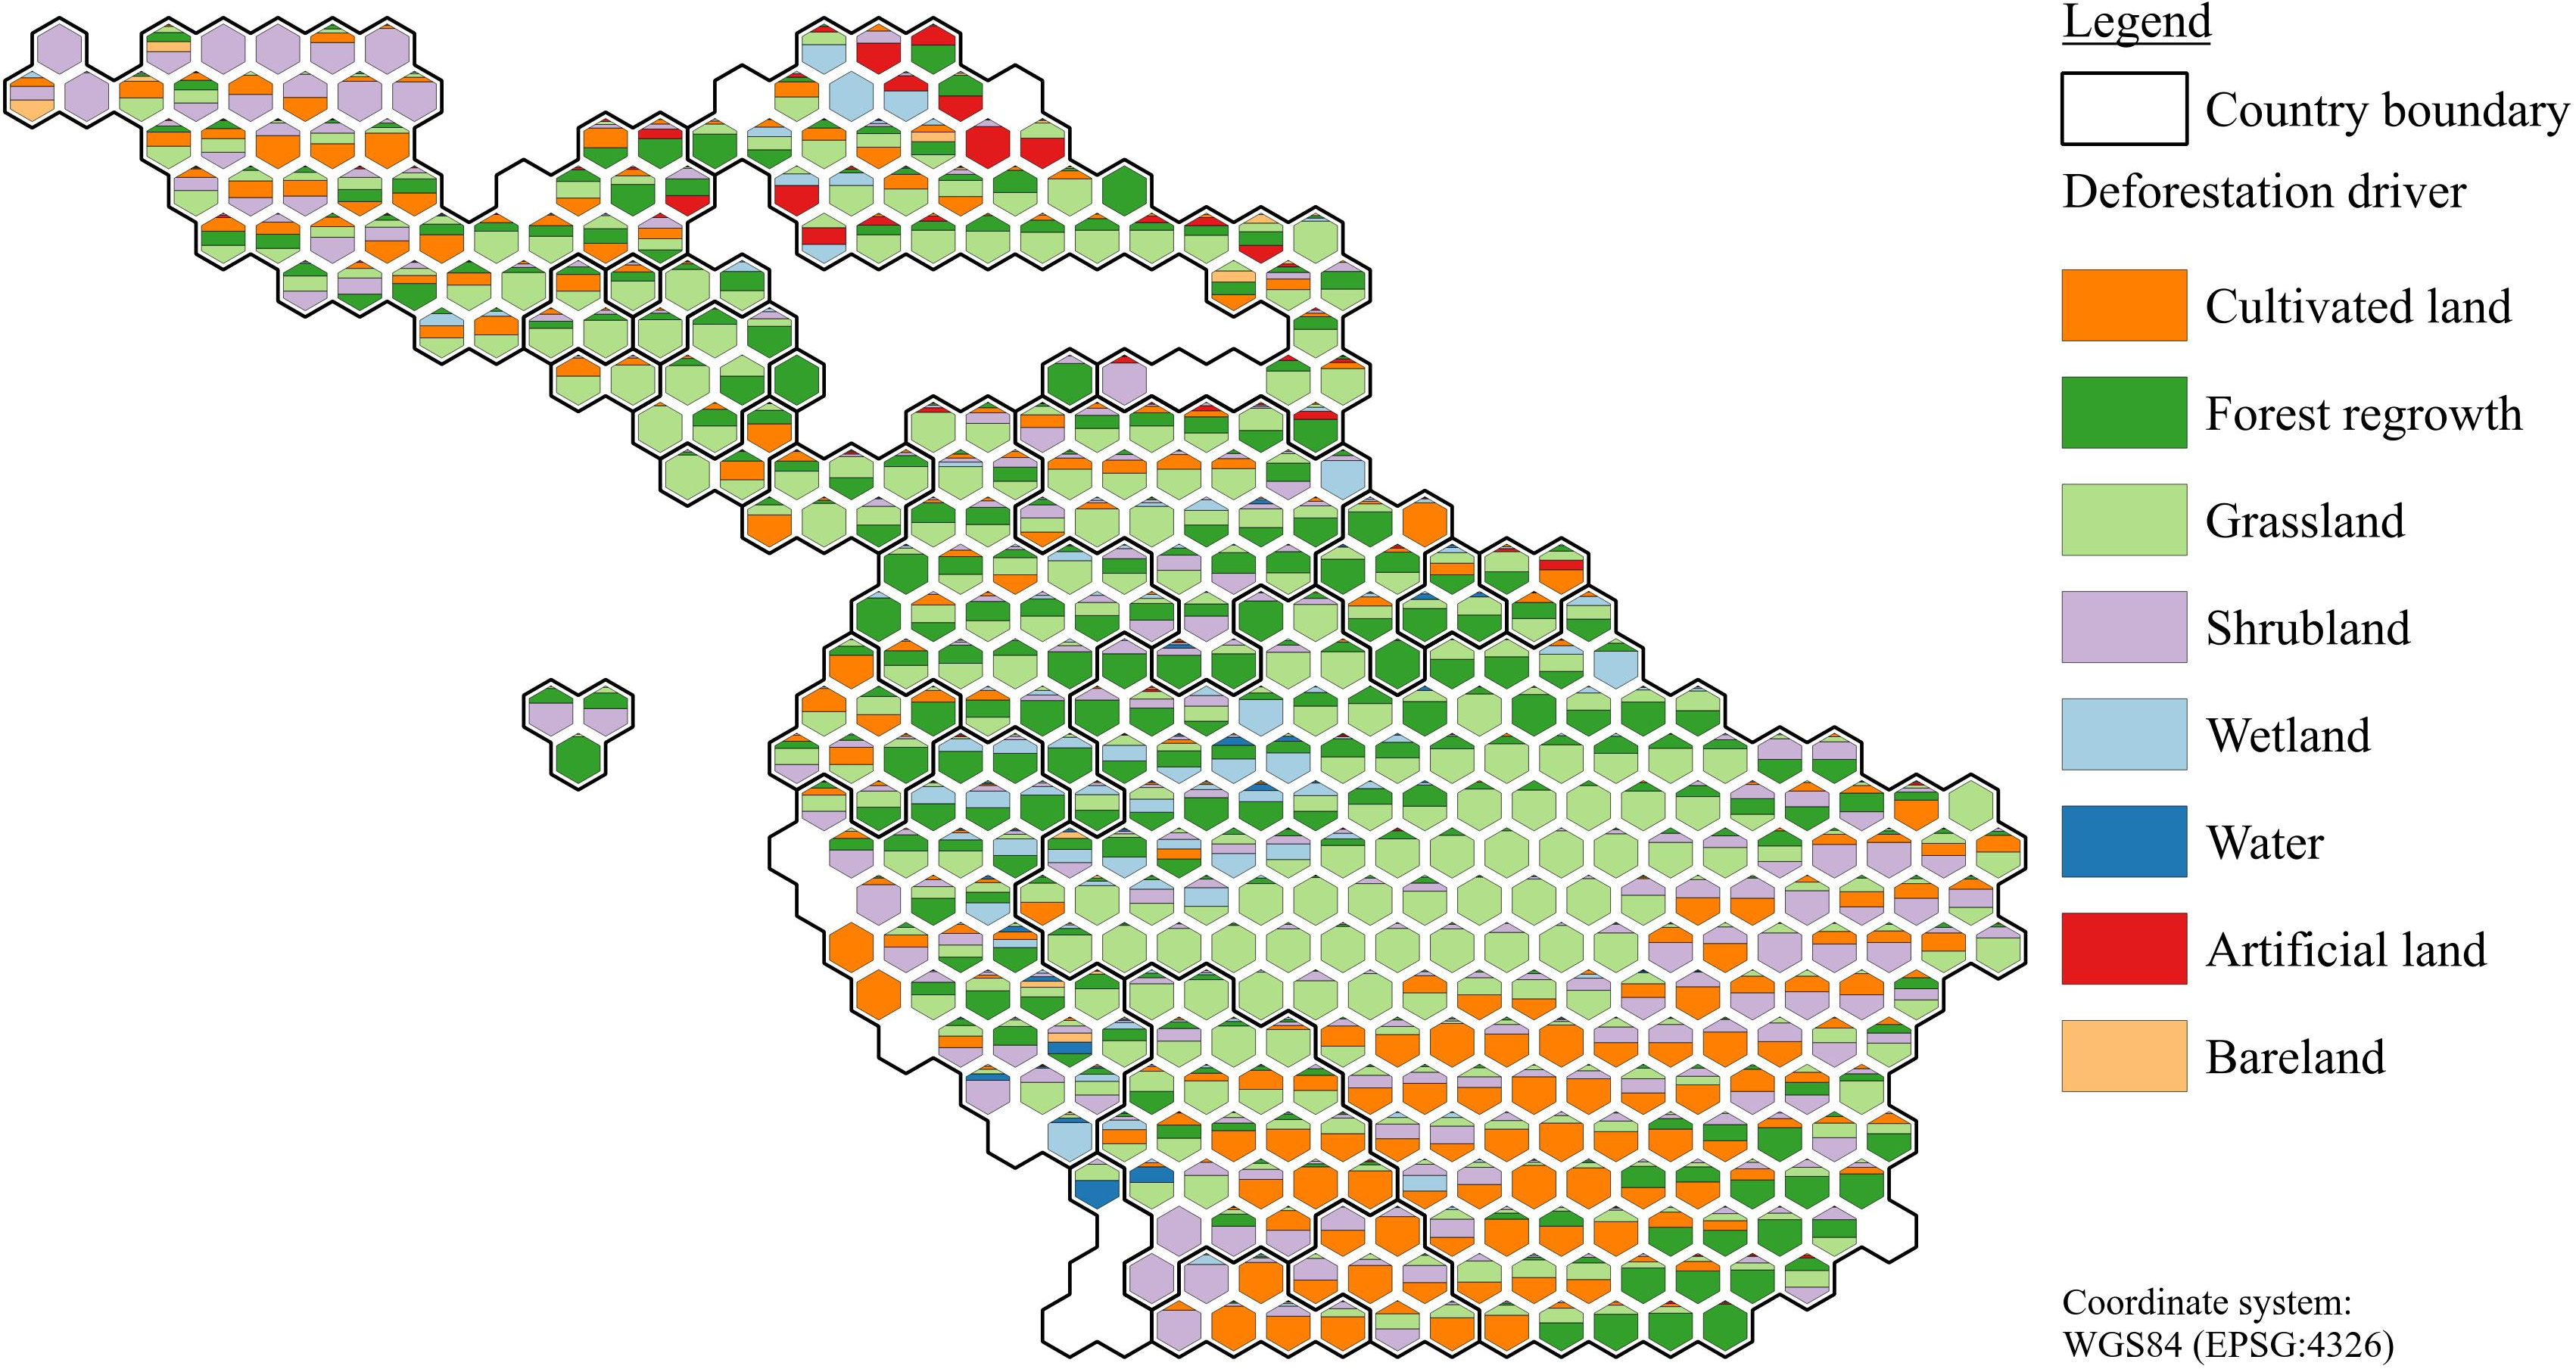
\includegraphics[scale=1]{img/americas_driver_frameless}
%				\caption[Ecosystem service values]{}
%				\label{fig:americasdriver}
%			\end{figure}

% ASIA
%			\begin{figure}[ht]
%				\centering
%				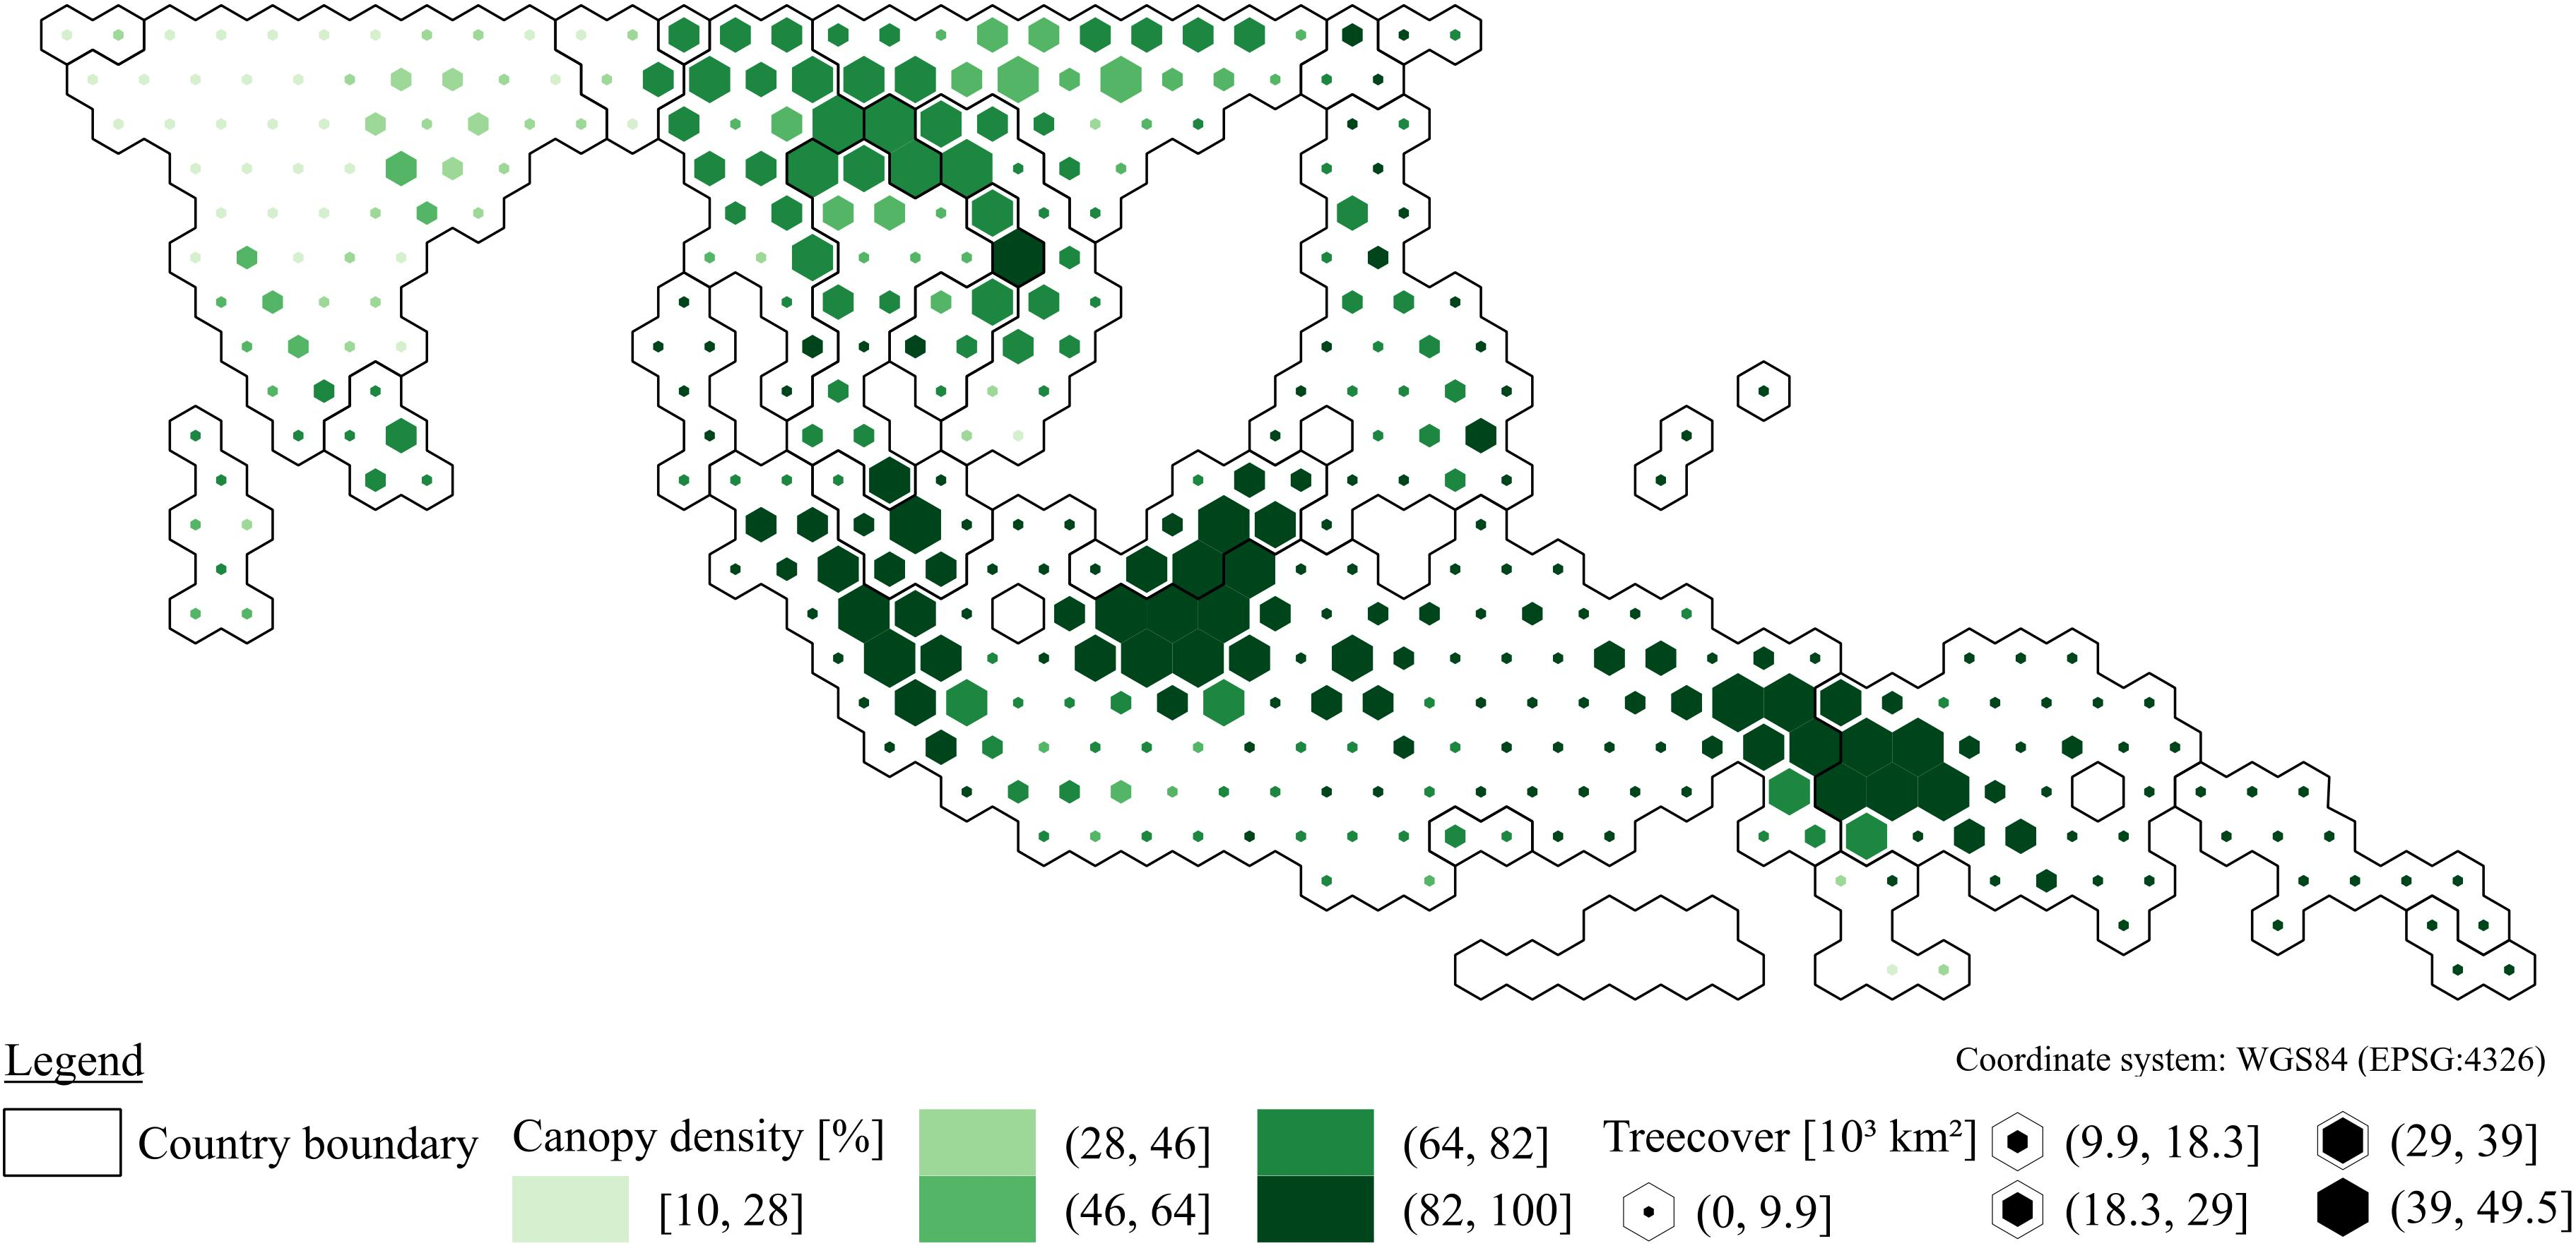
\includegraphics[scale=1]{img/asia_treecover_frameless}
%				\caption[Ecosystem service values]{}
%				\label{fig:asiacover}
%			\end{figure}
%			\begin{figure}[ht]
%				\centering
%				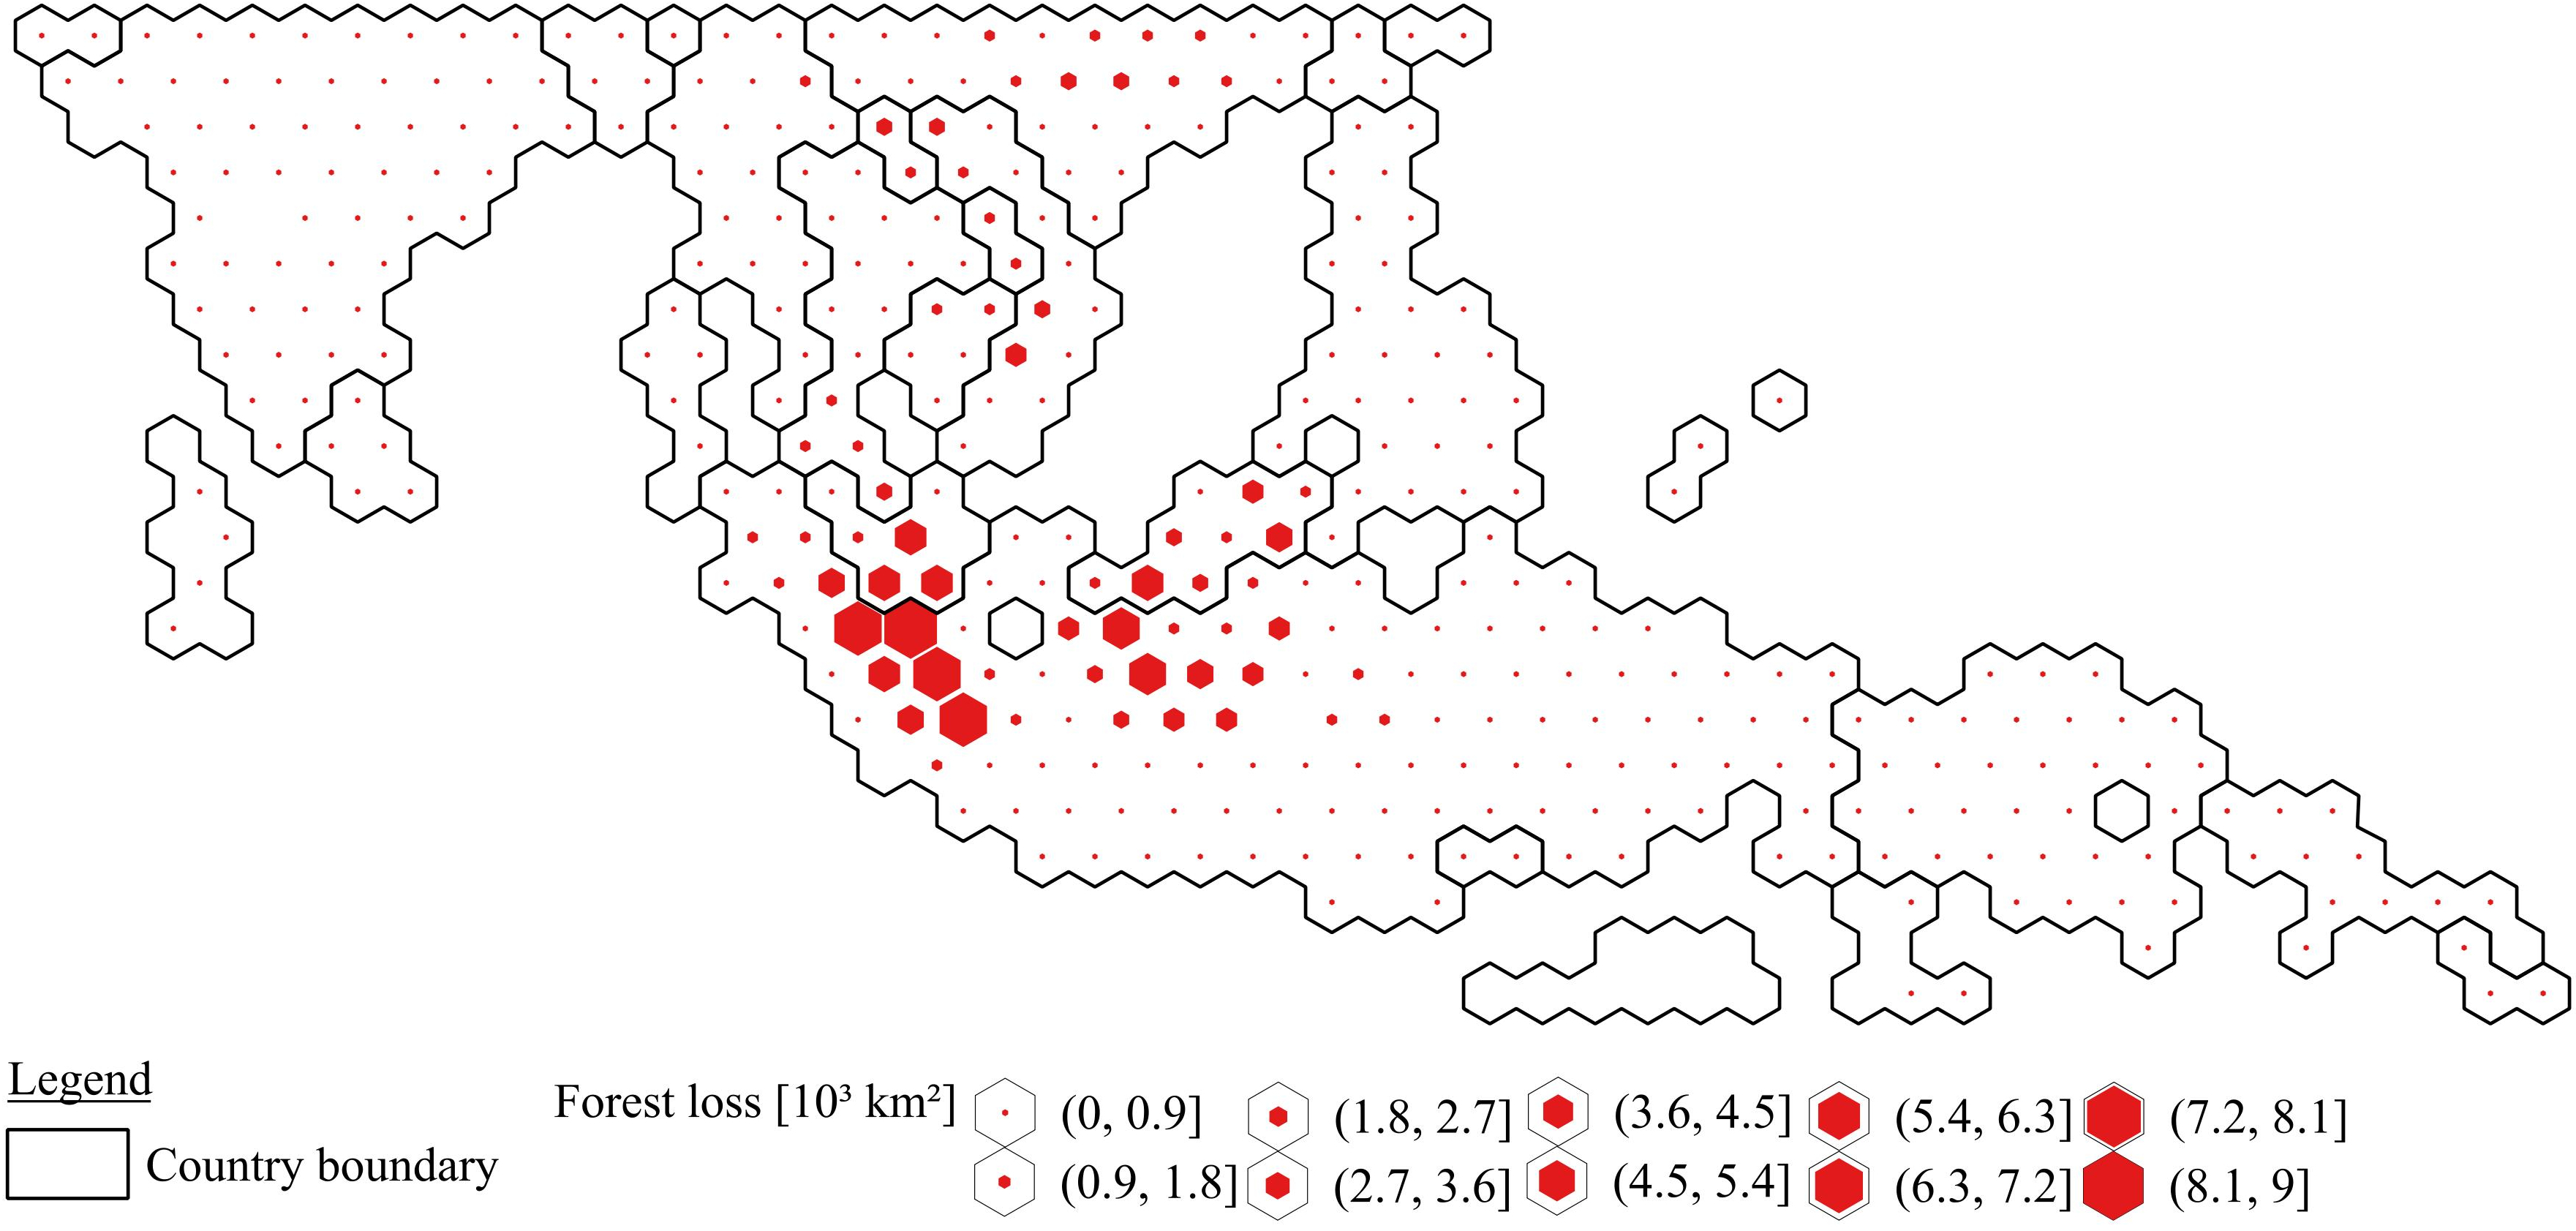
\includegraphics[scale=1]{img/asia_loss_frameless}
%				\caption[Ecosystem service values]{}
%				\label{fig:asialoss}
%			\end{figure}
%			\begin{figure}[ht]
%				\centering
%				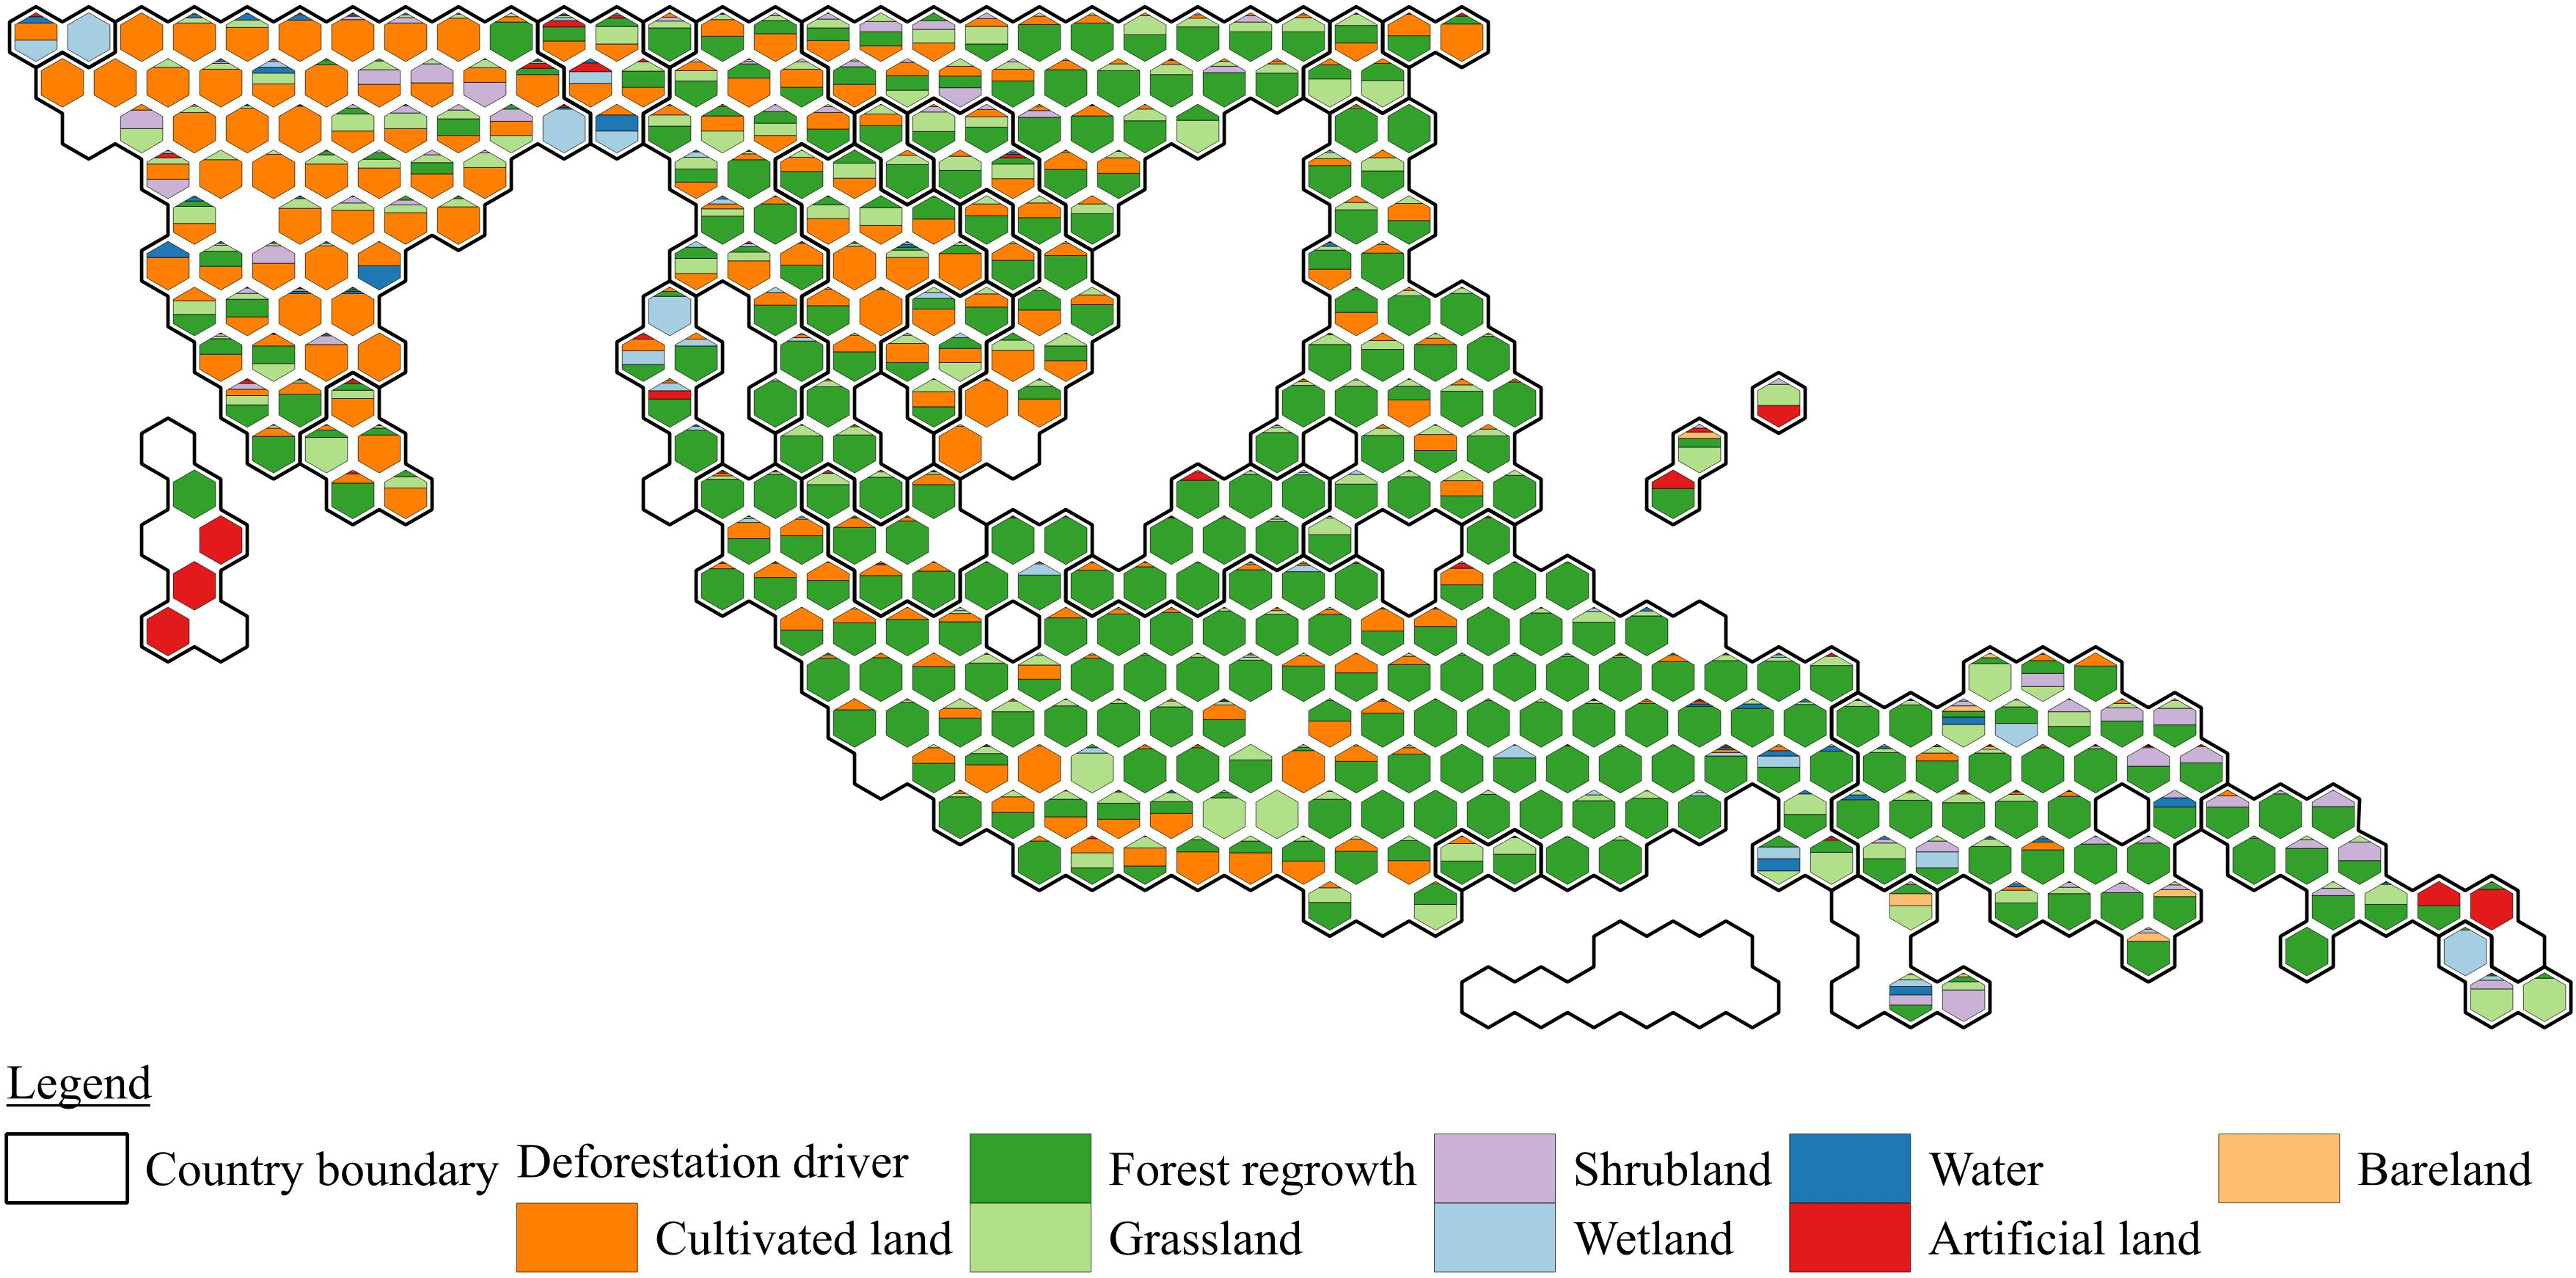
\includegraphics[scale=1]{img/asia_driver_frameless}
%				\caption[Ecosystem service values]{}
%				\label{fig:asiadriver}
%			\end{figure}

% AFRICA
%			\begin{figure}[ht]
%				\centering
%				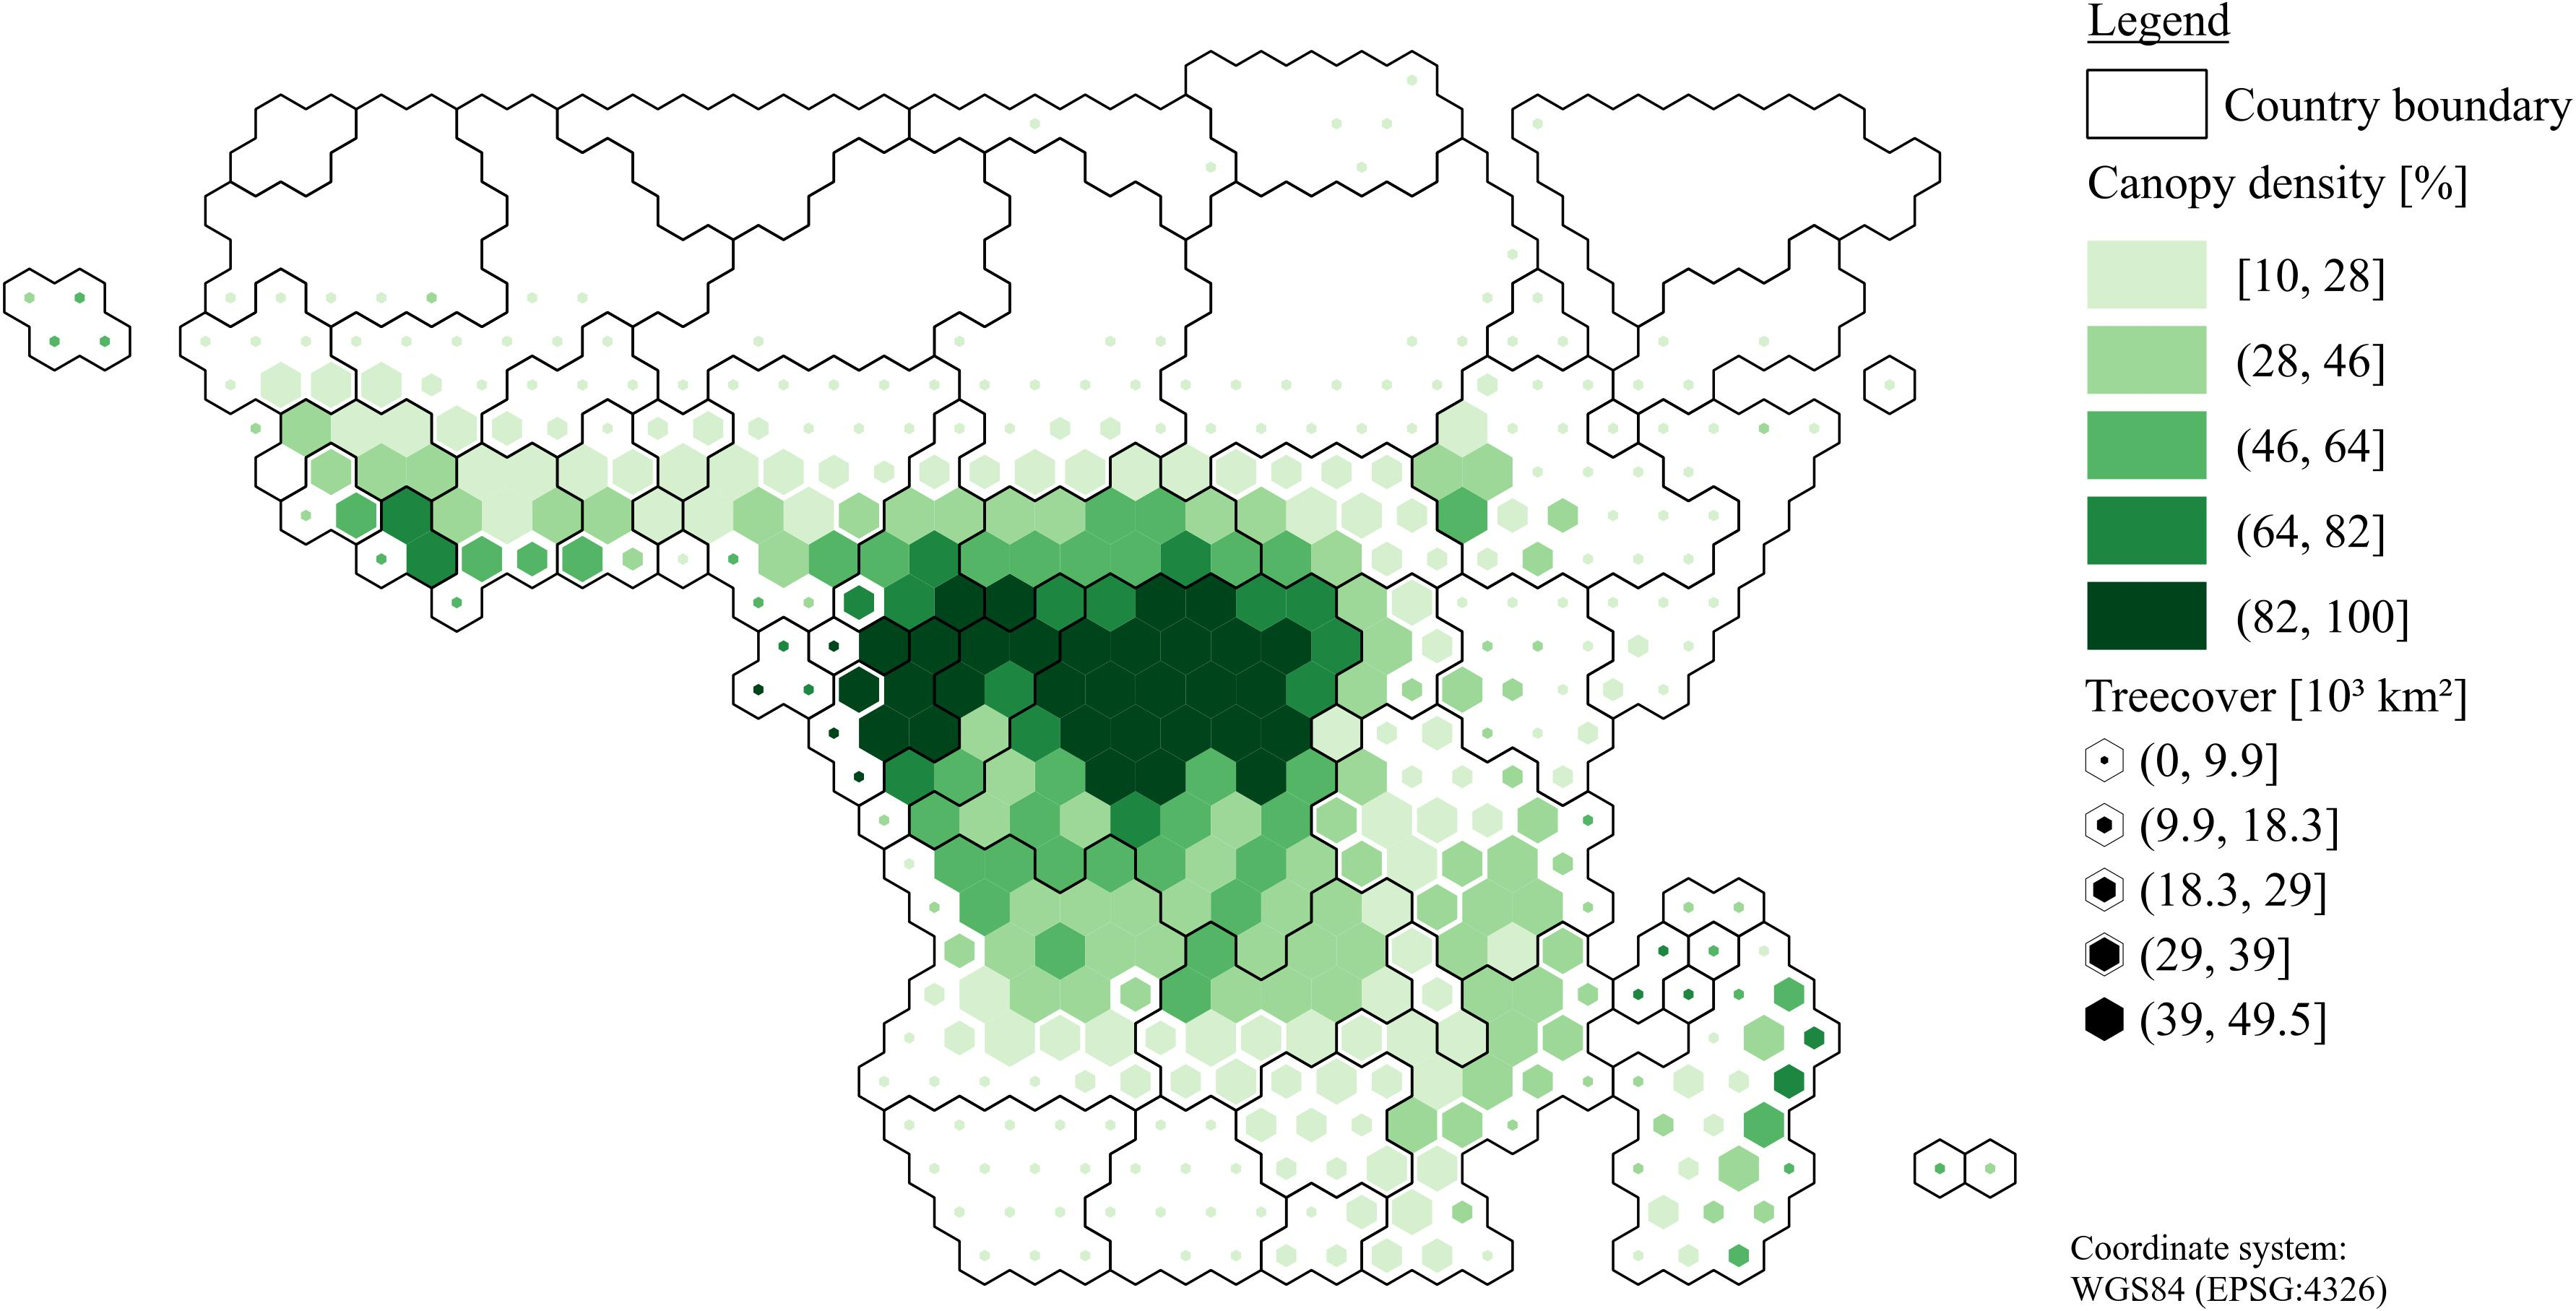
\includegraphics[scale=1]{img/africa_treecover_frameless}
%				\caption[Ecosystem service values]{}
%				\label{fig:africacover}
%			\end{figure}
%			\begin{figure}[ht]
%				\centering
%				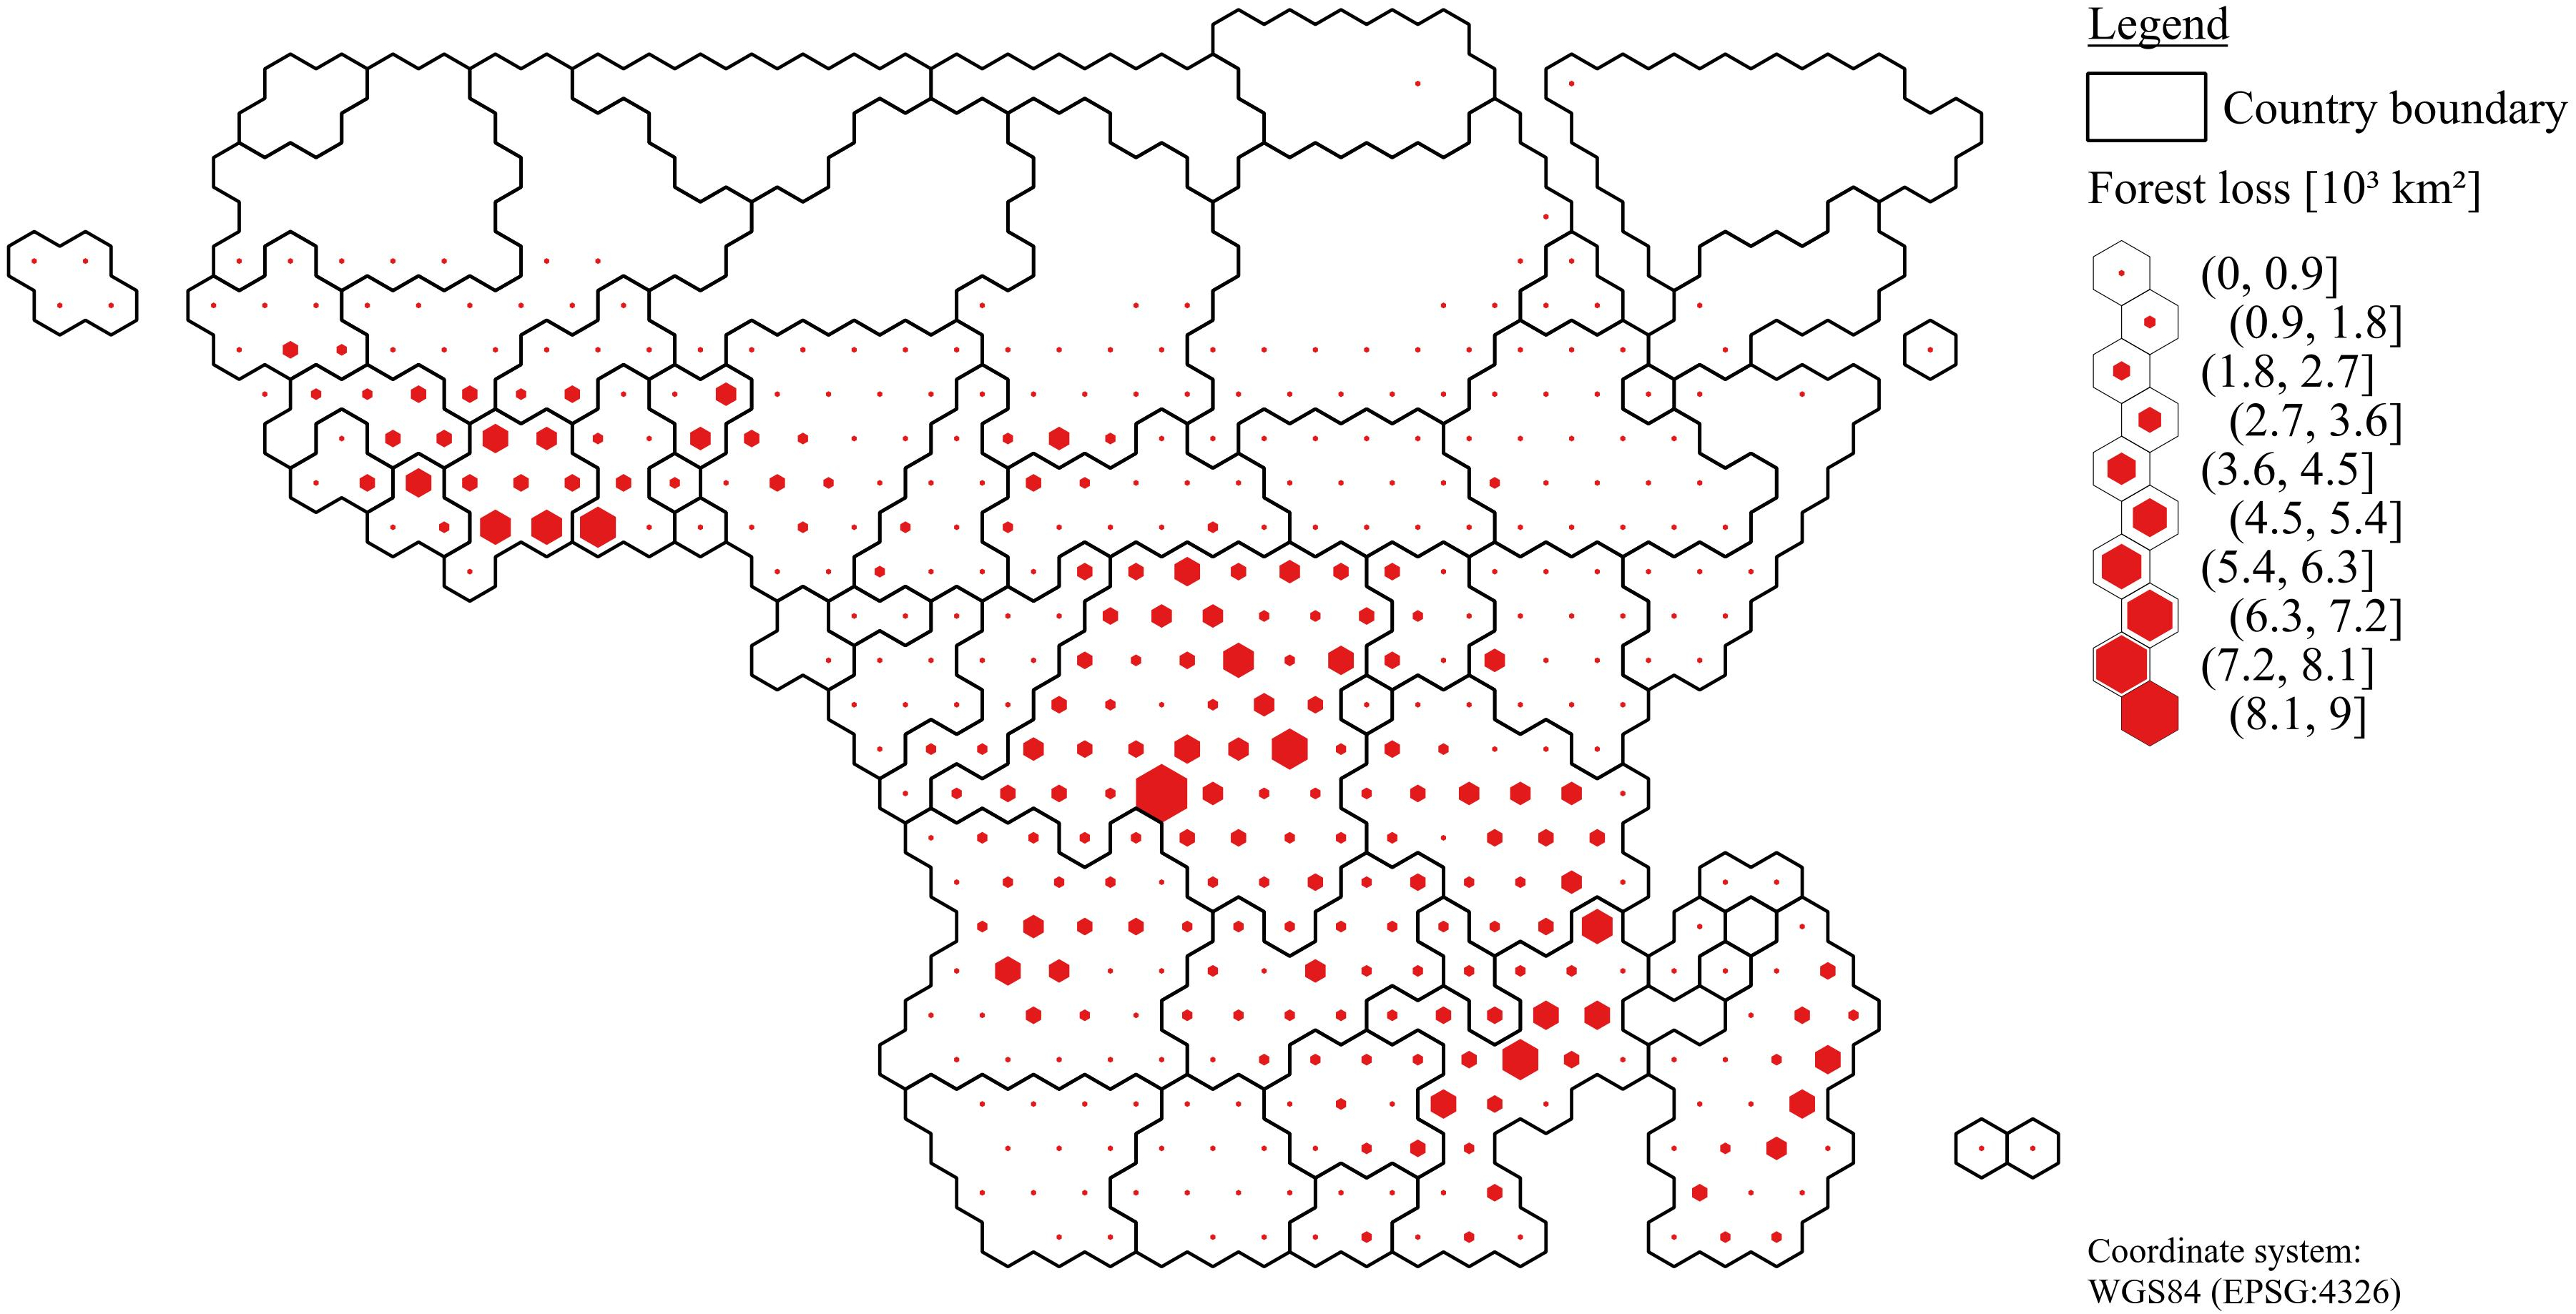
\includegraphics[scale=1]{img/africa_loss_frameless}
%				\caption[Ecosystem service values]{}
%				\label{fig:africaloss}
%			\end{figure}
%			\begin{figure}[ht]
%				\centering
%				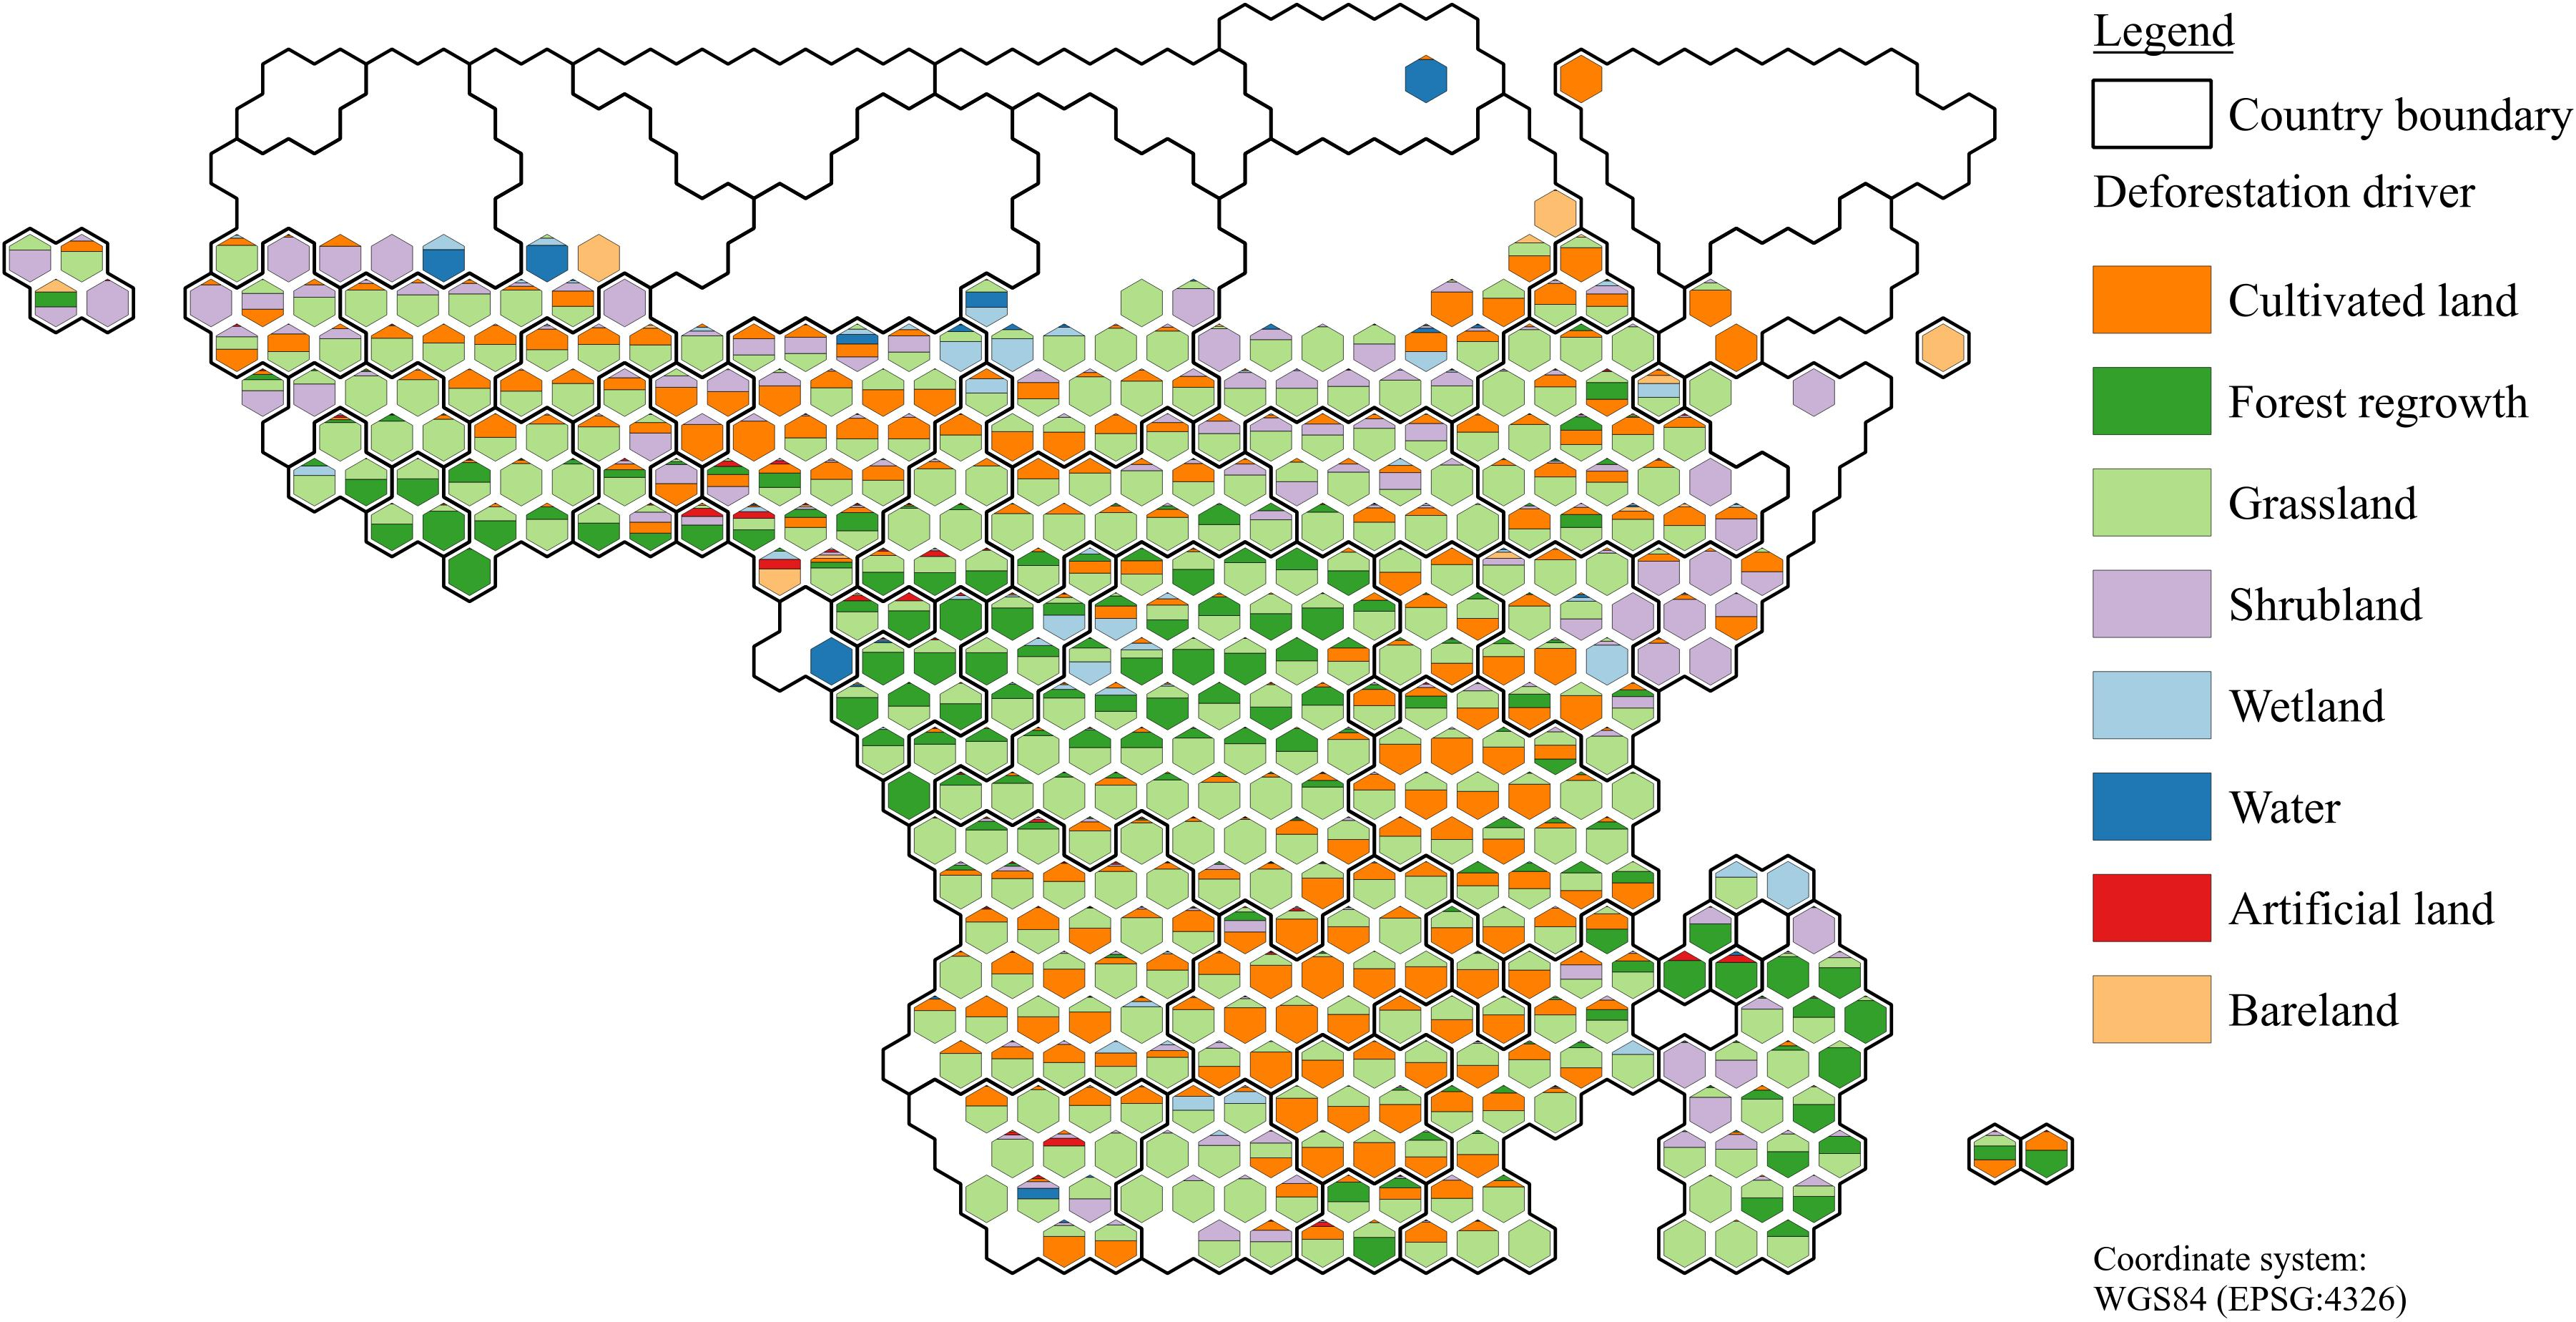
\includegraphics[scale=1]{img/africa_driver_frameless}
%				\caption[Ecosystem service values]{}
%				\label{fig:africadriver}
%			\end{figure}


% EMISSIONS
%		\begin{figure}[ht]
%			\centering
%			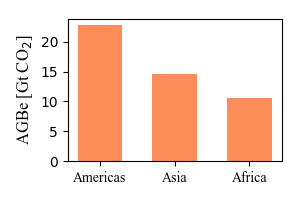
\includegraphics[scale=1]{img/agbe}
%			\caption[Ecosystem service values]{}
%			\label{fig:agbe}
%		\end{figure}
%		\begin{figure}[ht]
%			\centering
%			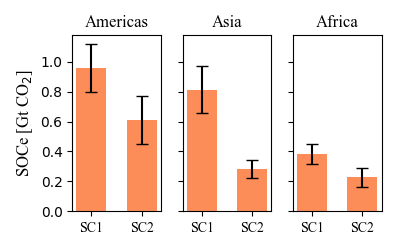
\includegraphics[scale=1]{img/soce}
%			\caption[Ecosystem service values]{}
%			\label{fig:soce}
%		\end{figure}
%
%		\begin{table}[ht]
%			\centering
%			\caption[Soil organic carbon emissions]{Soil organic carbon emissions}
%			\label{tab:soce_tab}
%			\begin{tabular}{lrrrrrrrrr}
%				\hline
%				\multirow{3}{*}{Region} & \multicolumn{3}{c}{SC1}& \multicolumn{3}{c}{SC2} & \multicolumn{3}{c}{SC3} \\
%				& \multicolumn{3}{c}{[Gt CO$_2$]}& \multicolumn{3}{c}{[Gt CO$_2$]} & \multicolumn{3}{c}{[Gt CO$_2$]} \\
%				& min & mean & max & min & mean & max & min & mean & max \\\hline
%				Americas & 0.80 & 0.96 & 1.12 & 0.45 & 0.61 & 0.77 & 0.43 & 0.59 & 0.76 \\
%				Asia & 0.66 & 0.81 & 0.97 & 0.22 & 0.28 & 0.34 & 0.22 & 0.28 & 0.33 \\
%				Africa & 0.32 & 0.39 & 0.45 & 0.17 & 0.23 & 0.29 & 0.16 & 0.23 & 0.29 \\\hline
%			\end{tabular}
%		\end{table}


% ESV
%		\begin{figure}[ht]
%			\centering
%			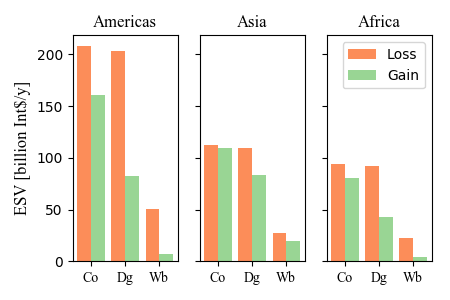
\includegraphics[scale=1]{img/esv}
%			\caption[Ecosystem service values]{}
%			\label{fig:esv}
%		\end{figure}


